%! TeX program = lualatex
\documentclass[12pt,a4paper]{article}

\usepackage[nil]{babel}
\usepackage{unicode-math}
\usepackage[svgnames]{xcolor}
\usepackage{lmodern}
\usepackage{graphicx}
\usepackage{wrapfig}
\usepackage{float}
\usepackage{parskip}
\usepackage{hyperref}
\usepackage{listings}
\usepackage{easytable}
\usepackage{fullpage}
\usepackage[font=small,labelfont=bf]{caption}

\definecolor{codegreen}{rgb}{0,0.6,0}
\definecolor{codegray}{rgb}{0.5,0.5,0.5}
\definecolor{codepurple}{rgb}{0.58,0,0.82}
\definecolor{backcolour}{rgb}{0.95,0.95,0.92}

\lstdefinestyle{mystyle}{
    backgroundcolor=\color{backcolour},   
    commentstyle=\color{codegreen},
    keywordstyle=\color{magenta},
    numberstyle=\tiny\color{codegray},
    stringstyle=\color{codepurple},
    basicstyle=\ttfamily\footnotesize,
    breakatwhitespace=false,         
    breaklines=true,                 
    captionpos=b,                    
    keepspaces=true,                 
    numbers=left,                    
    numbersep=5pt,                  
    showspaces=false,                
    showstringspaces=false,
    showtabs=false,                  
    tabsize=2
}


\lstset{style=mystyle}



\babelprovide[import=el, main, onchar=ids fonts]{greek} % can also do import=el-polyton
\babelprovide[import, onchar=ids fonts]{english}

\babelfont{rm}
          [Language=Default]{Liberation Sans}
\babelfont[english]{rm}
          [Language=Default]{Liberation Sans}
\babelfont{sf}
          [Language=Default]{Liberation Sans}
\babelfont{tt}
          [Language=Default]{Liberation Sans}


\setlength{\emergencystretch}{3em}

%Enter Title Here
\title{Εξόρυξη Δεδομένων και Αλγόριθμοι Μάθησης\\Εργαστηριακή Άσκηση 2022-2023}
\author{Λένος Χρίστου (ΑΜ: 1063014)\\Γρηγόρης Καπαδούκας (ΑΜ: 1072484)}

\begin{document}

\maketitle

%Insert Body Here
\setcounter{section}{-1}
\section{Αναλυτική Καταγραφή του Περιβάλλοντος Υλοποίησης}

\subsection{Καταγραφή Βιβλιοθηκών που Χρησιμοποιήθηκαν}
Για να υλοποιήσουμε την εργασία χρησιμοποιήσαμε γλώσσα προγραμματισμού\\ Python, όπως ζητείται στην εκφώνηση, με τις εξής κύριες βιβλιοθήκες:

\begin{itemize}
    \item Numpy
    \item Pandas
    \item Matplotlib
    \item Scikit-learn
    \item Tensorflow
    \item Scipy
    \item Seaborn
    \item Jupytext (για τη προαιρετική χρήση Jupyter Notebook)
\end{itemize}

\subsection{Αναλυτικά Βήματα για την Δημιουργία Πανομοιότυπου Περιβάλλοντος Υλοποίησης}
Παρακάτω δίνουμε αναλυτικά βήματα για την εγκατάσταση των βιβλιοθηκών σε ένα Python virtual environment, έτσι ώστε το περιβάλλον υλοποίησης να είναι πανομοιότυπο με αυτό που χρησιμοποιήσαμε εμείς:

\begin{enumerate}
    \item Εγκατάσταση του Miniconda μέσω του installer στη σελίδα:

        \textcolor{blue}{\href{https://docs.conda.io/en/latest/miniconda.html}{https://docs.conda.io/en/latest/miniconda.html}}

         Το Miniconda είναι μια δωρεάν μινιμαλιστική πλατφόρμα με cross-platform υποστήριξη που περιέχει το εργαλείο conda, με σκοπό την εύκολη δημιουργία και διαχείριση των Python virtual environments.

         Τα virtual environments αποτελούν ένα "απομονωμένο χώρο" όπου μπορούμε να εγκαταστήσουμε και να χρησιμοποιήσουμε κάποια συγκεκριμένη έκδοση της Python και βιβλιοθήκες της, χωρίς να επηρεάσουμε τυχόν εγκατάσταση της Python που βρίσκεται ήδη στο σύστημα. 

         Εναλλακτική επιλογή που μπορεί να χρησιμοποιηθεί στη θέση του Miniconda είναι το Anaconda. Το Miniconda αναφέρεται επειδή το προτιμήσαμε εμείς στην χρήση μας.

     \item Δημιουργία του conda virtual environment με αυτόματη εγκατάσταση των βιβλιοθηκών που επιθυμούμε μέσω της εκτέλεση της εξής εντολής στον φάκελο της εργασίας σε τερματικό (ή command prompt αντίστοιχα σε πλατφόρμα Windows):

         \begin{lstlisting}[language=Bash]
conda env create -f environment.yml\end{lstlisting}

\textbf{Παρατήρηση:} Στο δικό μας περιβάλλον χρησιμοποιήσαμε τη βιβλιοθήκη Tensorflow ρυθμισμένο για GPU support, με σκοπό την υλοποίηση των RNN. Εάν δεν επιθυμείτε να χρησιμοποιήσετε GPU support μπορείτε να αφαιρέσετε από το παραπάνω αρχεία τις γραμμές που αντιστοιχούν στα πακέτα που περιέχουν 'nvidia' στο όνομά τους.

     \item Η εγκατάσταση των βιβλιοθηκών στο virtual environment έχει ολοκληρωθεί, οπότε τώρα θα φορτώσουμε το environment με την εξής εντολή:
         \begin{lstlisting}[language=Bash]
conda activate venv\end{lstlisting}
\item \textbf{(Προαιρετικό):} Για τη ρύθμιση του GPU support για το Tensorflow, θα χρειαστεί να εκτελεστούν οι παρακάτω εντολές:
         \begin{lstlisting}[language=Bash]
CUDNN_PATH=$(dirname $(python -c "import nvidia.cudnn;print(nvidia.cudnn.__file__)"))
export LD_LIBRARY_PATH=$LD_LIBRARY_PATH:$CONDA_PREFIX/lib/:$CUDNN_PATH/lib
mkdir -p $CONDA_PREFIX/etc/conda/activate.d
echo 'CUDNN_PATH=$(dirname $(python -c "import nvidia.cudnn;print(nvidia.cudnn.__file__)"))' >> $CONDA_PREFIX/etc/conda/activate.d/env_vars.sh
echo 'export LD_LIBRARY_PATH=$LD_LIBRARY_PATH:$CONDA_PREFIX/lib/:$CUDNN_PATH/lib' >> $CONDA_PREFIX/etc/conda/activate.d/env_vars.sh
\end{lstlisting}
    Για παραπάνω πληροφορίες σχετικά με το GPU support και για τον έλεγχο σωστής λειτουργίας του και επίλυση τυχόν προβλημάτων μεταβείτε στην official σελίδα οδηγιών του Tensorflow:

        \textcolor{blue}{\href{https://www.tensorflow.org/install/pip}{https://www.tensorflow.org/install/pip}}

    \item Τώρα πλέον είμαστε έτοιμοι και μπορούμε να εκτελέσουμε τον κώδικα απευθείας στο τερματικό ή μέσω του Jupyter Notebook:

        Για να εκτελέσουμε απευθείας τον κώδικα στο environment εκτελούμε απλά την εξής εντολή:
         \begin{lstlisting}[language=Bash]
python Code/<filename>.py\end{lstlisting}

        Για να εκτελέσουμε το Jupyter Notebook στο environment εκτελούμε την εξής εντολή στο τερματικό:
         \begin{lstlisting}[language=Bash]
jupyter notebook\end{lstlisting}
\end{enumerate}

\section{Υλοποίηση και Αποτελέσματα Ερωτήματος 1}

\subsection{Σύντομη Περιγραφή της Διαδικασίας Υλοποίησης}

Για την υλοποίηση του ερωτήματος αυτού, αναφέρουμε αρχικά ότι χρησιμοποιούμε την βιβλιοθήκη Pandas για το διάβασμα και την χρήστη του data.csv αρχείου με τα δεδομένα μας.

Έπειτα χρησιμοποιώντας την μέθοδο describe() του Pandas τυπώνουμε σχετικά στατιστικά στοιχεία για τα δεδομένα κάθε στήλης, πιο συγκεκριμένα τιμές για το συνολικό άθροισμα ανά στήλη (count), μέση τιμή (mean), τυπική απόκλιση (std), ελάχιστη τιμή (min), τιμές 25\%, 50\%, 75\%, και μέγιστη τιμή (max). Στις τιμές αυτές στρογγυλοποιούμε στα δύο δεκαδικά ψηφία για το τύπωμα, ώστε να είναι πιο αναγνώσιμα. 

Ακόμα τυπώνουμε μέσω for λούπας ιστογράμματα για κάθε Series του Pandas DataFrame που περιέχει τα δεδομένα του dataset, με εξαίρεση τα Series 'Country' και 'Date', για τα οποία η προβολή ιστογράμματος δεν θα μας δώσει χρήσιμη πληροφορία. Με αυτόν τον τρόπο μπορούμε να καταλάβουμε την κατανομή των δεδομένων. Για τα ιστογράμματα χρησιμοποιούμε την παράμετρο "bins = 20" με σκοπόν να κάνουμε grouping των τιμών του άξονα x σε 20 ισομεγέθη bins στο εύρος τιμών που παίρνουν οι τιμές των εισαγωγών στο Series κάθε φορά. Αυτό είναι αναγκαίο επειδή πολύ συχνά τιμές εμφανίζονται μια μόνο φορά στα δεδομένα, οπότε αν δείξουμε αυτές τις τιμές χωρίς κανένα grouping δεν θα μπορούσαμε να λάβουμε αποτελέσματα σχετικά με την κατανομή της πιθανότητας των τιμών.

Τέλος με χρήση των βιβλιοθηκών Pandas, Seaborn και Matplotlib, υπολογίζουμε αρχικά το Correlation Matrix και έπειτα κάνουμε plot το Correlation Matrix Heatmap που προκύπτει από αυτό, έτσι ώστε να εμφανίζονται οι τίτλοι των Series στους άξονες x και y και να εμφανίζονται οι τιμές του correlation που προέκυψαν στο Correlation Matrix ως κελιά στο σημείο τομής οποιονδήποτε δύο κατηγοριών. Οι τιμές για το correlation ανήκουν στο εύρος [-1,1] με 1 να σημαίνει πλήρη συσχέτιση, 0 να σημαίνει καμία συσχέτιση και -1 να σημαίνει πλήρη αρνητική συσχέτιση (πχ αντιστρόφως ανάλογες τιμές).

\subsection{Τελικά Αποτελέσματα και Σχολιασμός τους}

\subsubsection{Τελικά Αποτελέσματα}
Παρακάτω παρουσιάζουμε ένα πίνακα με τα αποτελέσματα που προέκυψαν από την εκτέλεση της μεθόδου describe() του Pandas στο DataFrame του dataset:

\begin{table}[!ht]
    \centering
    \resizebox{\textwidth}{!}{\begin{tabular}{|c|c|c|c|c|c|c|c|c|c|c|c|c|}
    \hline
        \textbf{Value}
        & \textbf{Latitude}
        & \textbf{Longitude}
        & \multicolumn{1}{|p{2cm}|}{\centering \textbf{Average temperature per year}}
        & \multicolumn{1}{|p{2cm}|}{\centering \textbf{Hospital beds per 1000 people}}
        & \multicolumn{1}{|p{2cm}|}{\centering \textbf{Medical doctors per 1000 people}}
        & \multicolumn{1}{|p{2cm}|}{\centering \textbf{GDP / Capita}}
        & \textbf{Population}
        & \multicolumn{1}{|p{2cm}|}{\centering \textbf{Median age}}
        & \multicolumn{1}{|p{2cm}|}{\centering \textbf{Population aged 65 and over (\%)}}
        & \multicolumn{1}{|p{2cm}|}{\centering \textbf{Daily tests}}
        & \textbf{Cases}
        & \textbf{Deaths}
        \\ \hline
        count & 38472.0 & 38472.0 & 38472.0 & 38472.0 & 38472.0 & 38472.0 & 38472.0 & 38472.0 & 38472.0 & 30577.0 & 38218.0 & 34862.0 \\ \hline
        mean & 23.74 & 20.21 & 17.72 & 3.17 & 2.09 & 19002.33 & 48969829.03 & 32.75 & 10.66 & 39440.59 & 287902.66 & 8090.5 \\ \hline
        std & 26.06 & 61.07 & 8.13 & 2.56 & 1.52 & 22271.11 & 142725118.68 & 8.47 & 6.77 & 150184.66 & 1405242.87 & 29548.75 \\ \hline
        min & -40.9 & -106.35 & -2.0 & 0.2 & 0.02 & 411.6 & 341284.0 & 16.0 & 1.0 & -239172.0 & 1.0 & 1.0 \\ \hline
        25\% & 8.62 & -3.44 & 11.0 & 1.4 & 0.82 & 3659.0 & 4793900.0 & 27.0 & 5.0 & 1505.0 & 2074.0 & 77.0 \\ \hline
        50\% & 27.51 & 21.82 & 20.0 & 2.5 & 1.89 & 8821.8 & 11484636.0 & 32.0 & 8.0 & 5520.0 & 21431.0 & 527.0 \\ \hline
        75\% & 45.94 & 47.48 & 25.0 & 4.49 & 3.21 & 25946.2 & 42862958.0 & 41.0 & 16.0 & 20382.0 & 137377.0 & 3480.5 \\ \hline
        max & 64.96 & 179.41 & 29.0 & 13.05 & 7.52 & 114704.6 & 1339180127.0 & 48.0 & 28.0 & 2945871.0 & 28605669.0 & 513091.0 \\ \hline
    \end{tabular}}
    \caption{Στατιστικά Δεδομένα για κάθε Στήλη του Dataset} 
\end{table}

Οι τιμές αυτές φαίνονται και στο αρχείο "describe.csv" που συμπεριλαμβάνεται στον φάκελο "Report".

Παρακάτω φαίνονται επίσης τα ιστογράμματα της κάθε στήλης των δεδομένων του dataset που φτιάξαμε:

\begin{figure}[H]
	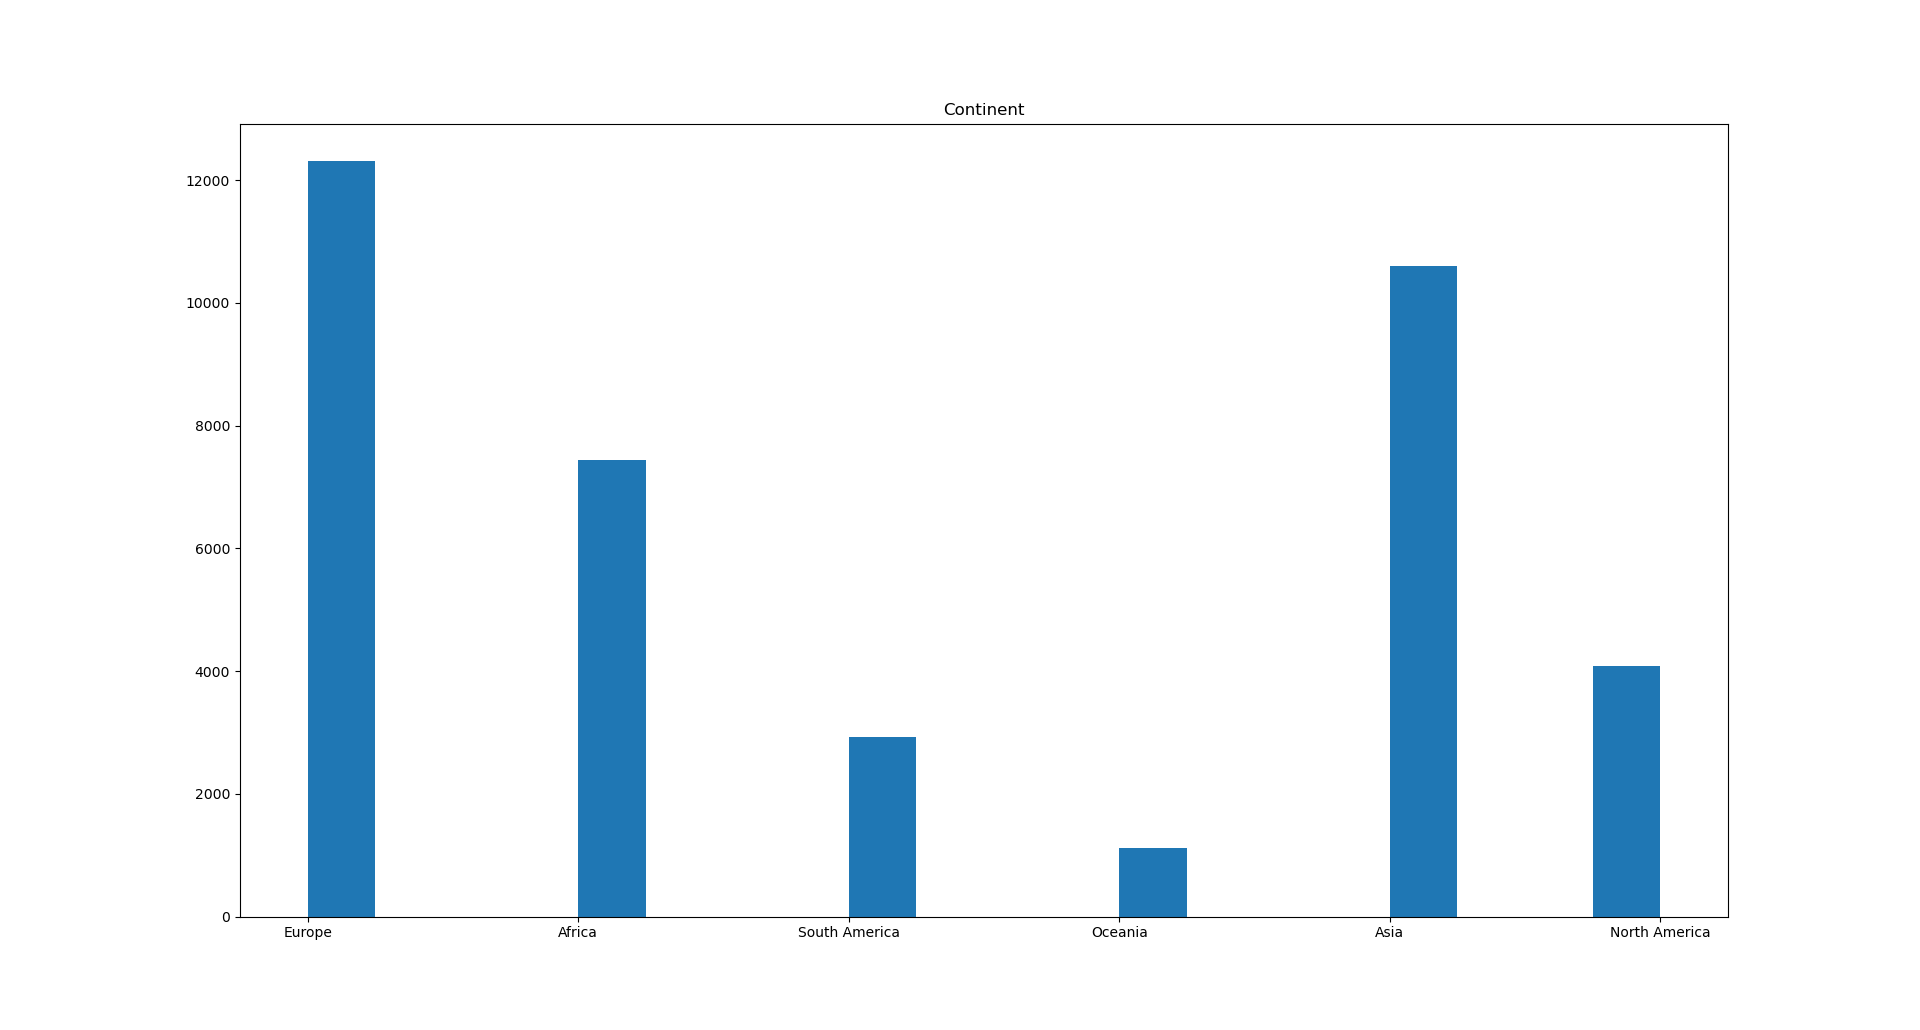
\includegraphics[width=\textwidth]{Figures/Question1/1. Histogram for Continent.png}
	\caption{Ιστόγραμμα για στήλη 'Continent'}
\end{figure}

\begin{figure}[H]
	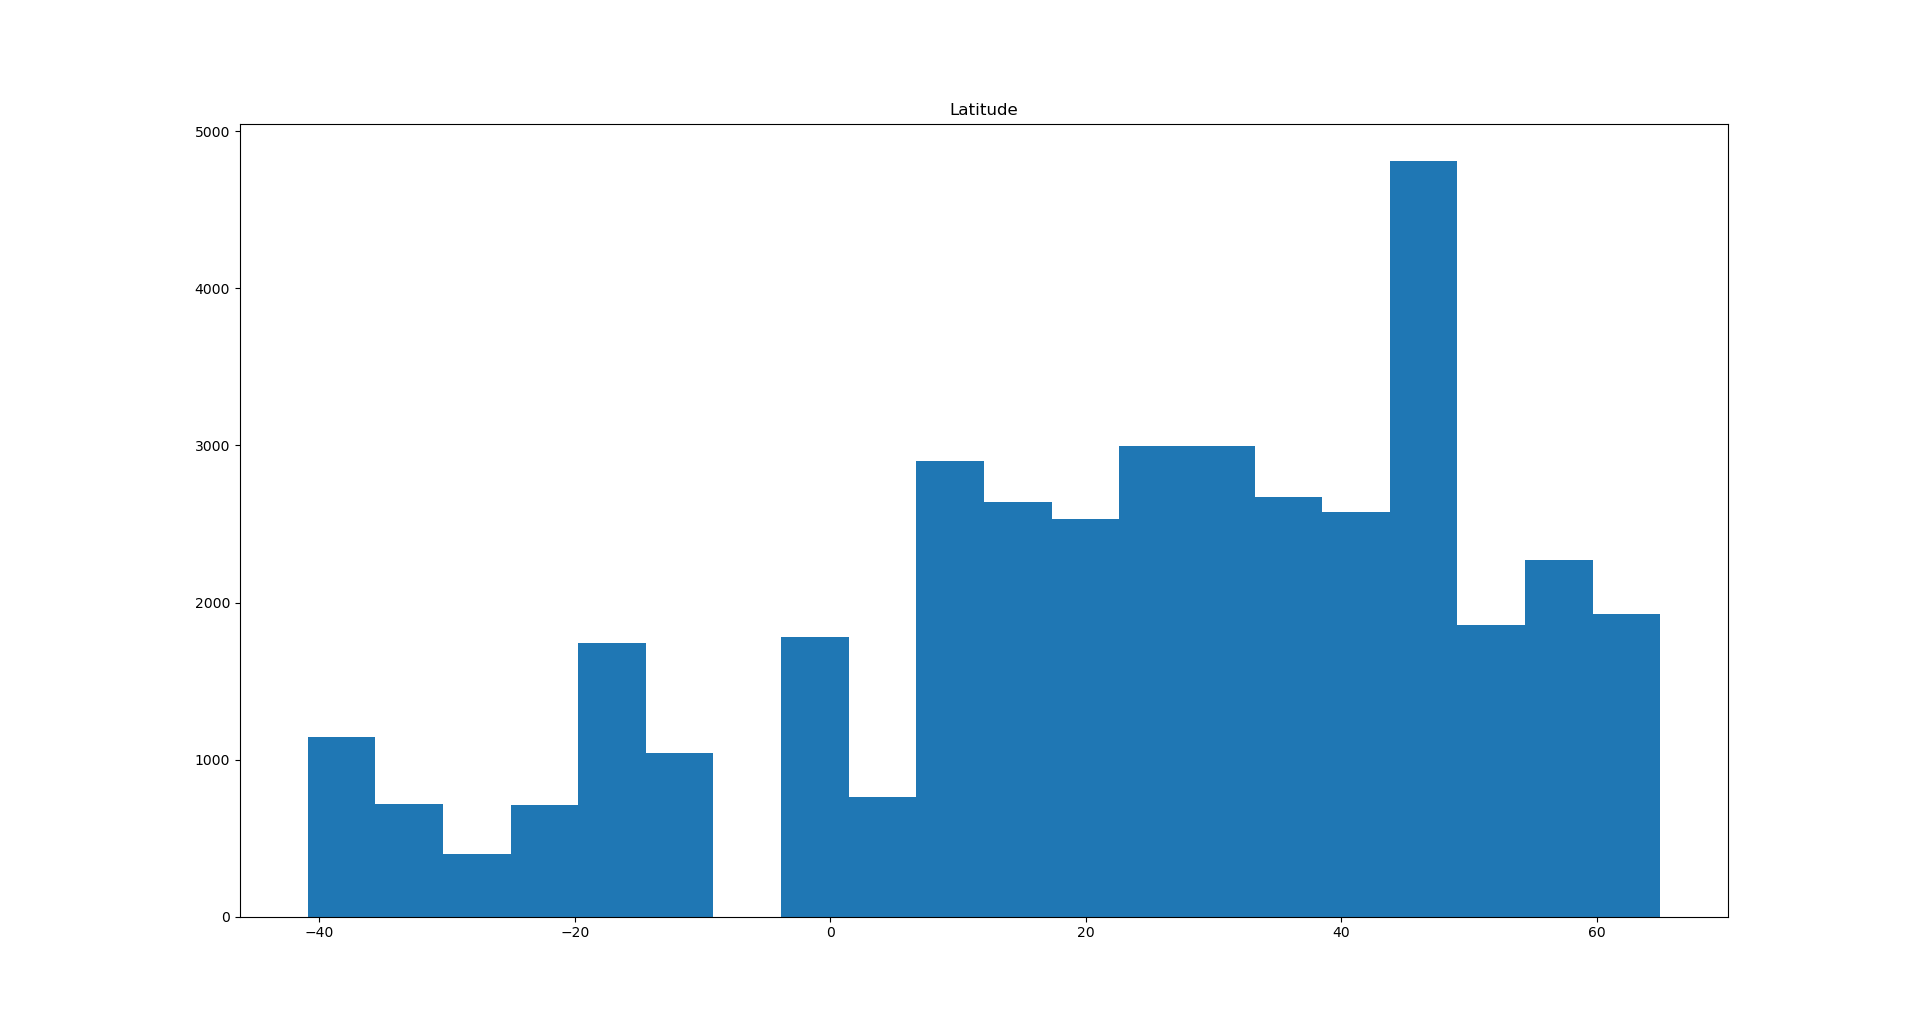
\includegraphics[width=\textwidth]{Figures/Question1/2. Histogram for Latitude.png}
	\caption{Ιστόγραμμα για στήλη 'Latitude'}
\end{figure}

\begin{figure}[H]
	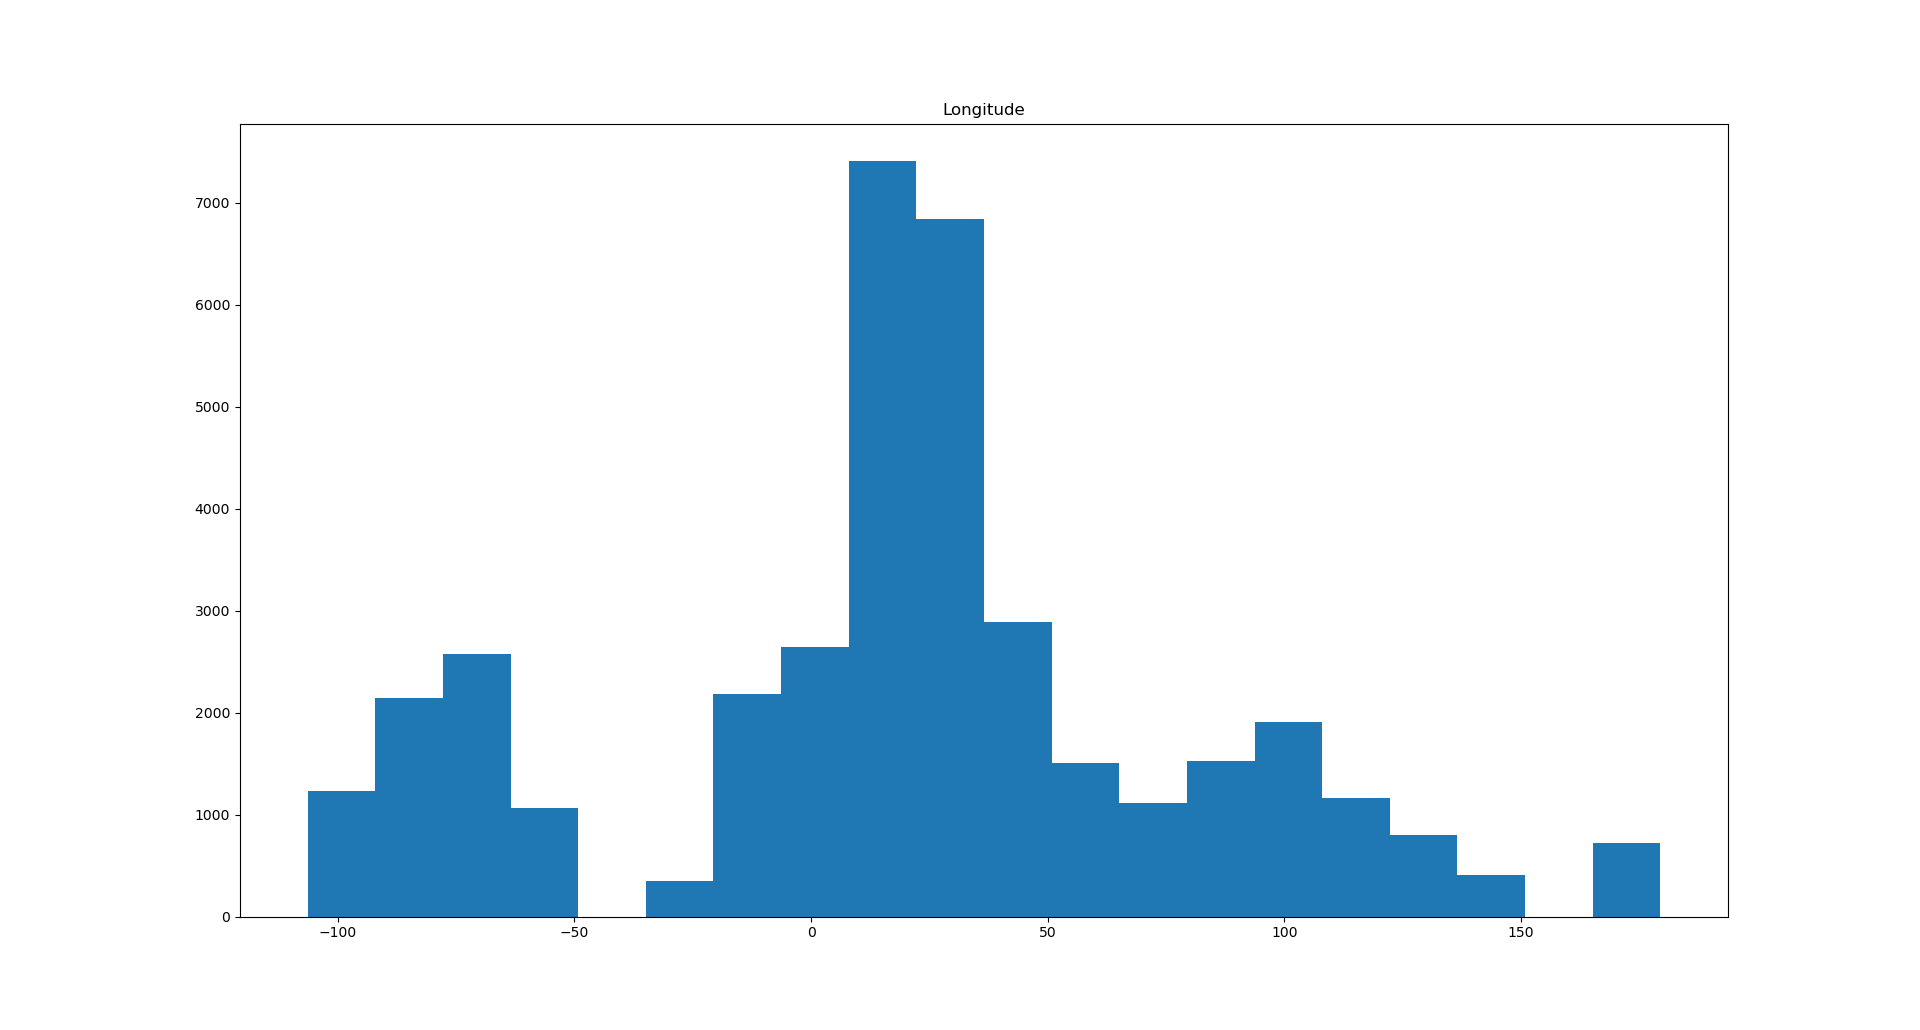
\includegraphics[width=\textwidth]{Figures/Question1/3. Histogram for Longtitude.png}
	\caption{Ιστόγραμμα για στήλη 'Longtitude'}
\end{figure}

\begin{figure}[H]
	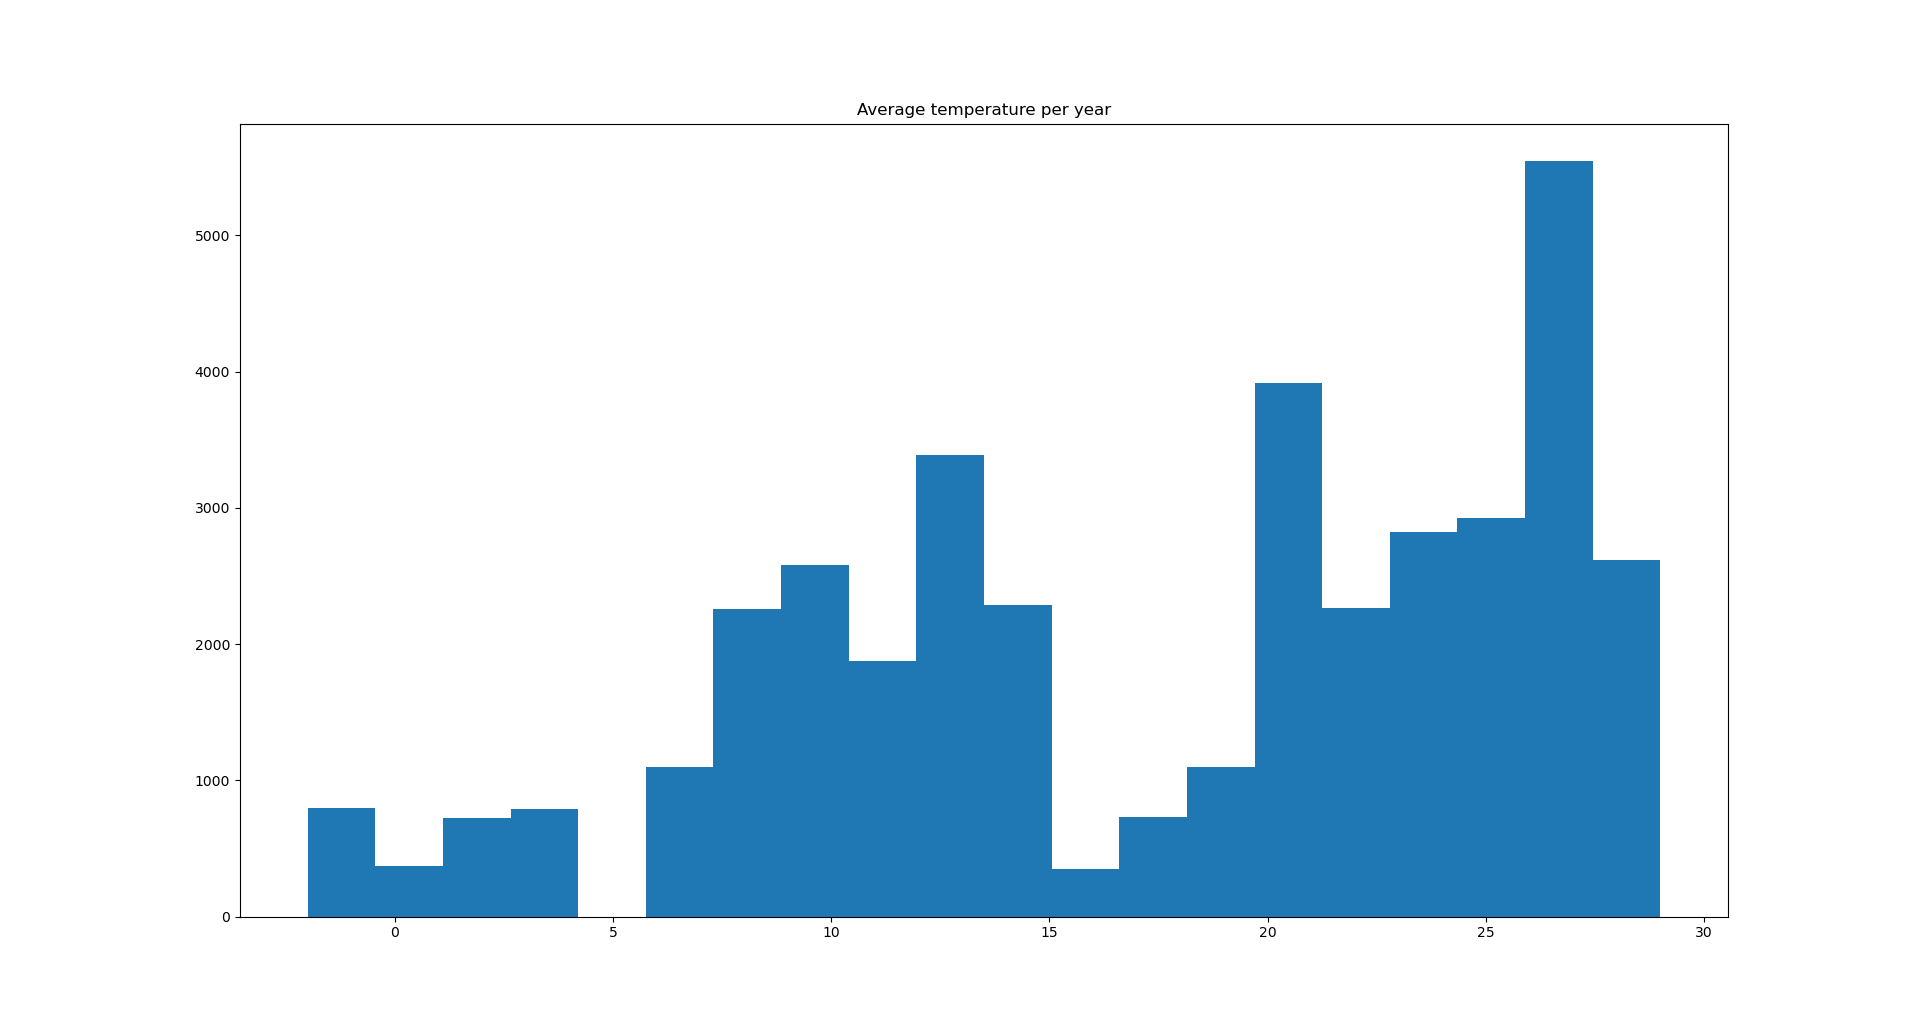
\includegraphics[width=\textwidth]{Figures/Question1/4. Histogram for average temperature per year.png}
	\caption{Ιστόγραμμα για στήλη 'Temperature'}
\end{figure}

\begin{figure}[H]
	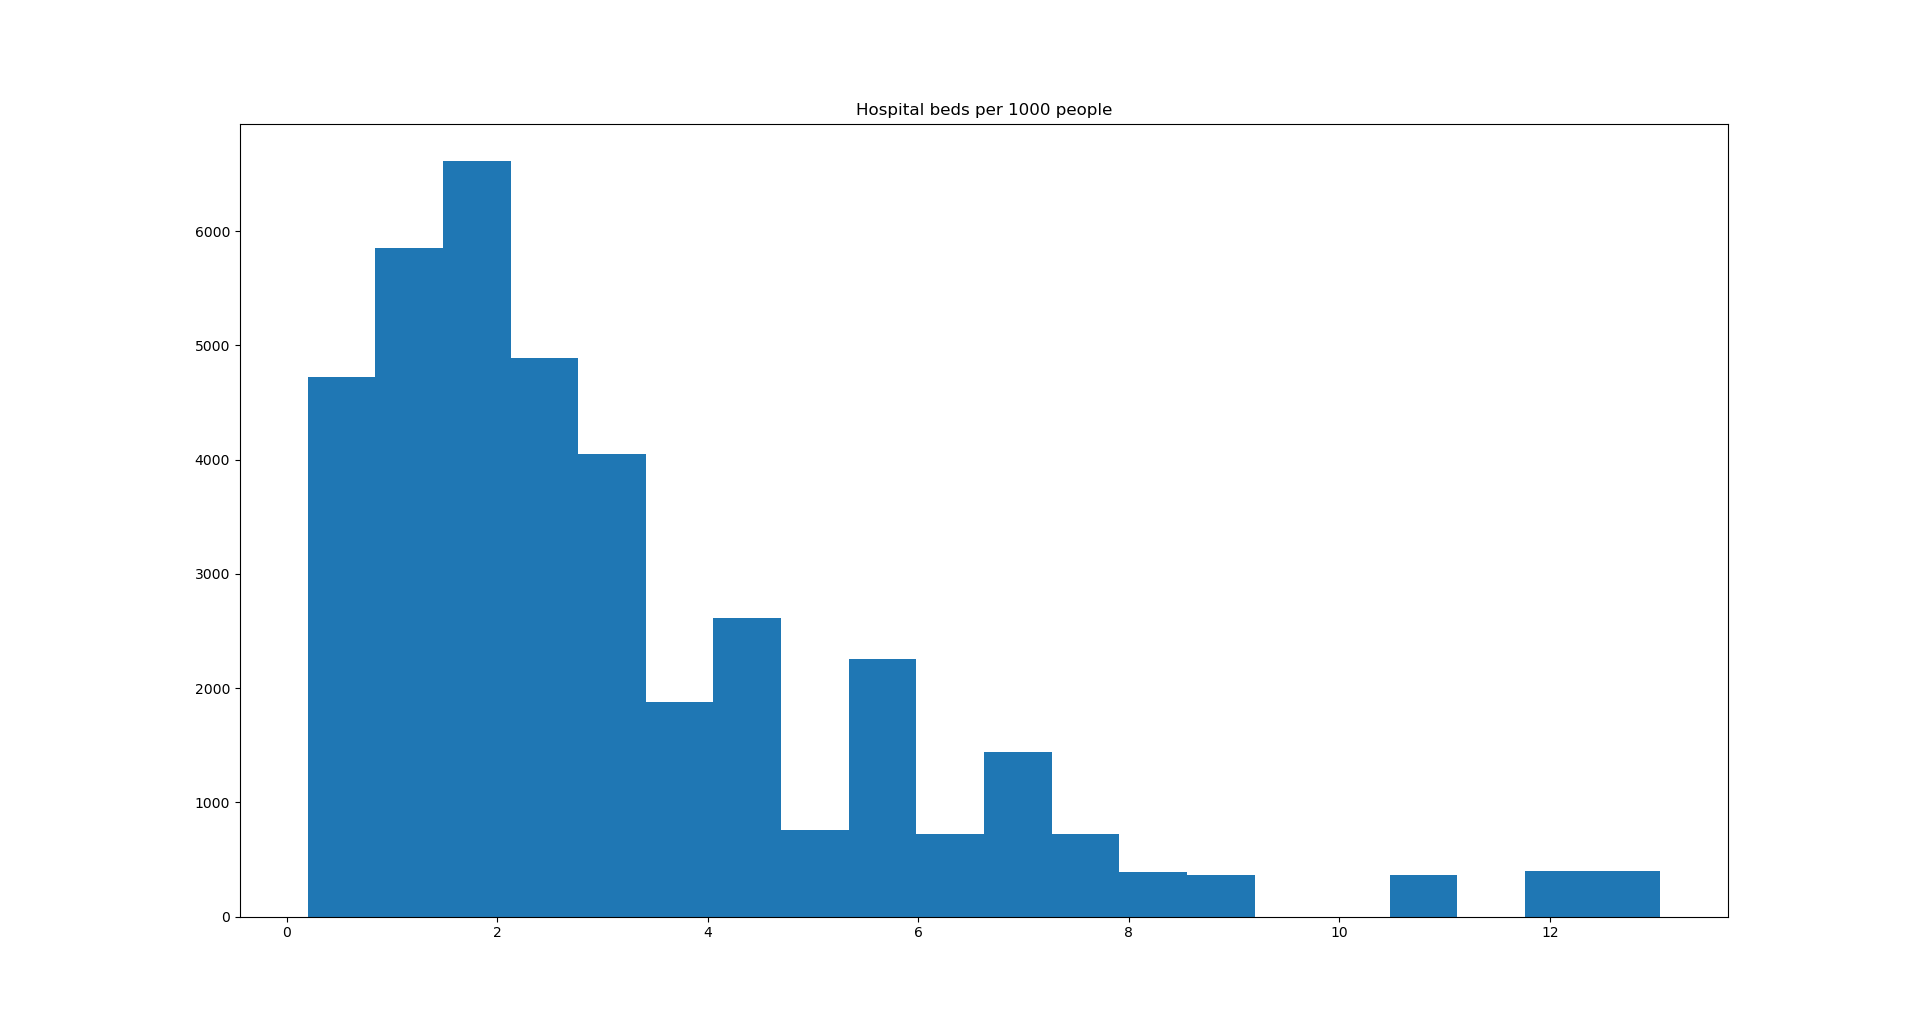
\includegraphics[width=\textwidth]{Figures/Question1/5. Histogram for hospital beds per 1000 people.png}
	\caption{Ιστόγραμμα για στήλη 'Hospital beds per 1000 people'}
\end{figure}

\begin{figure}[H]
	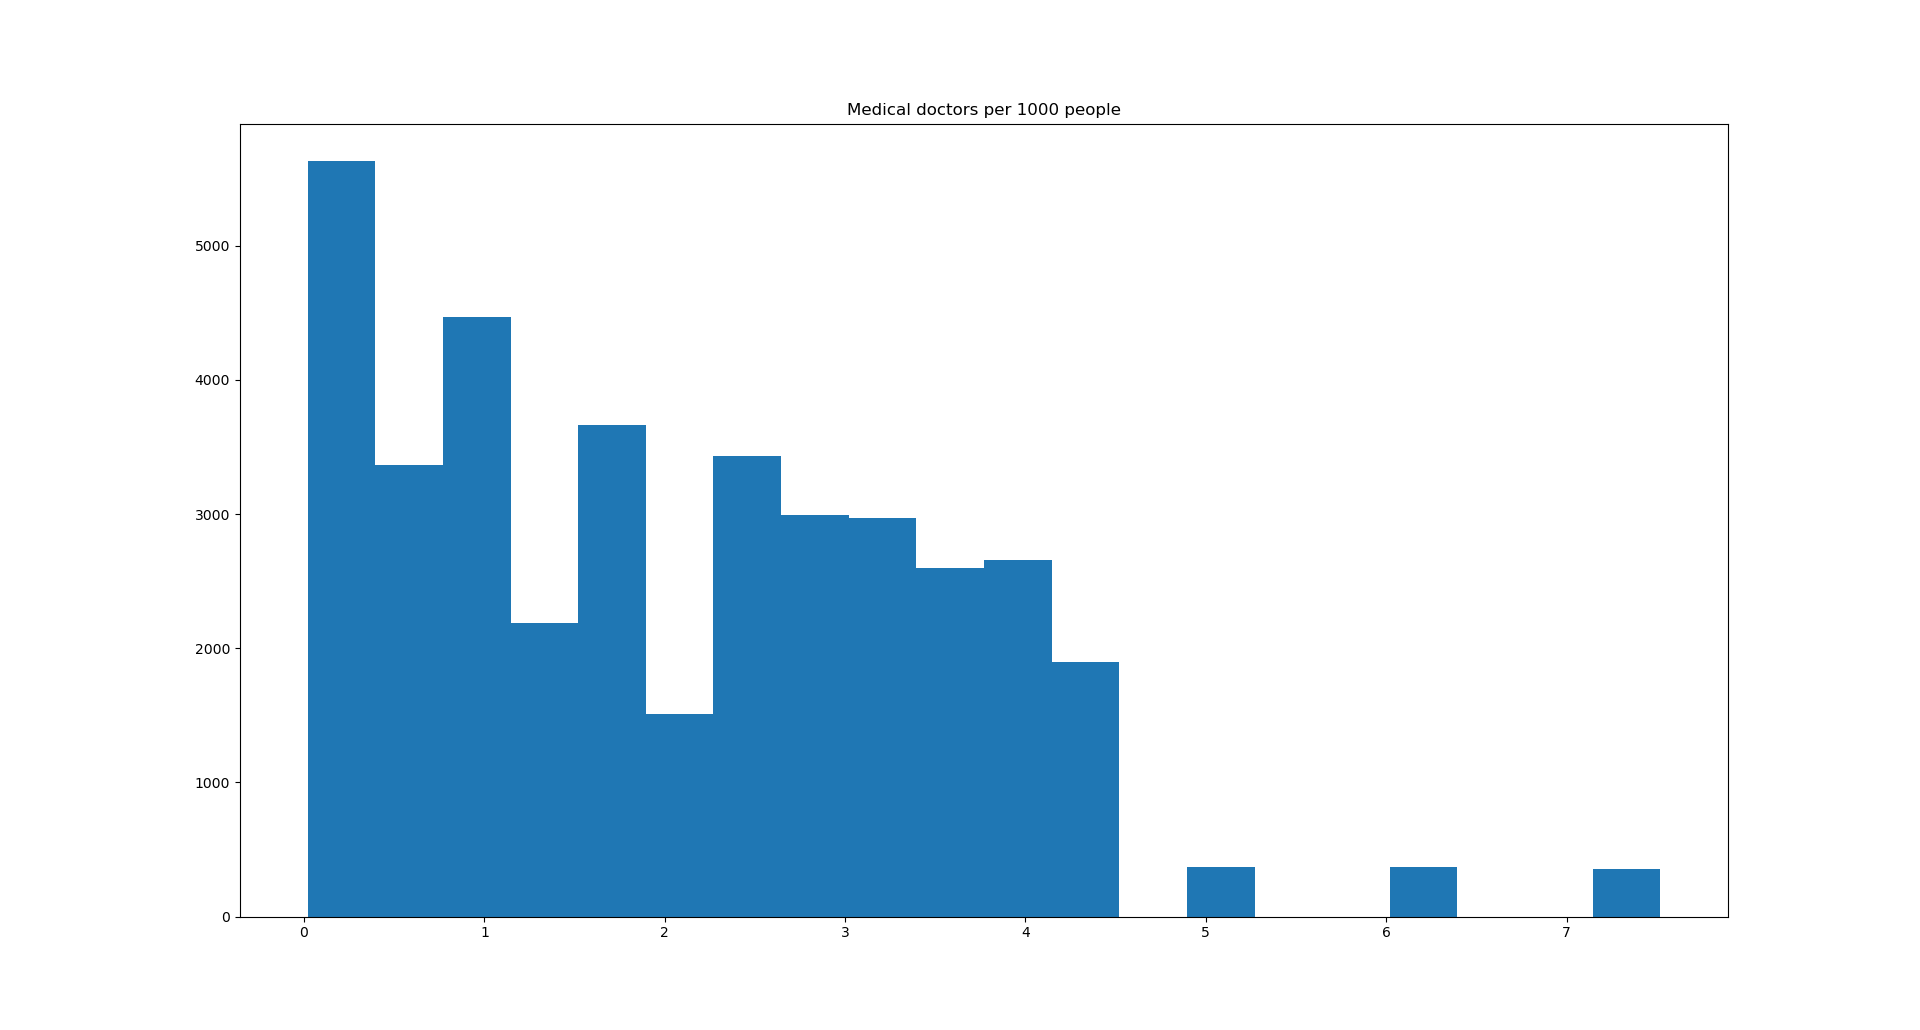
\includegraphics[width=\textwidth]{Figures/Question1/6. Histogram for medical doctors per 1000 people.png}
	\caption{Ιστόγραμμα για στήλη 'Medical doctors per 1000 people'}
\end{figure}

\begin{figure}[H]
	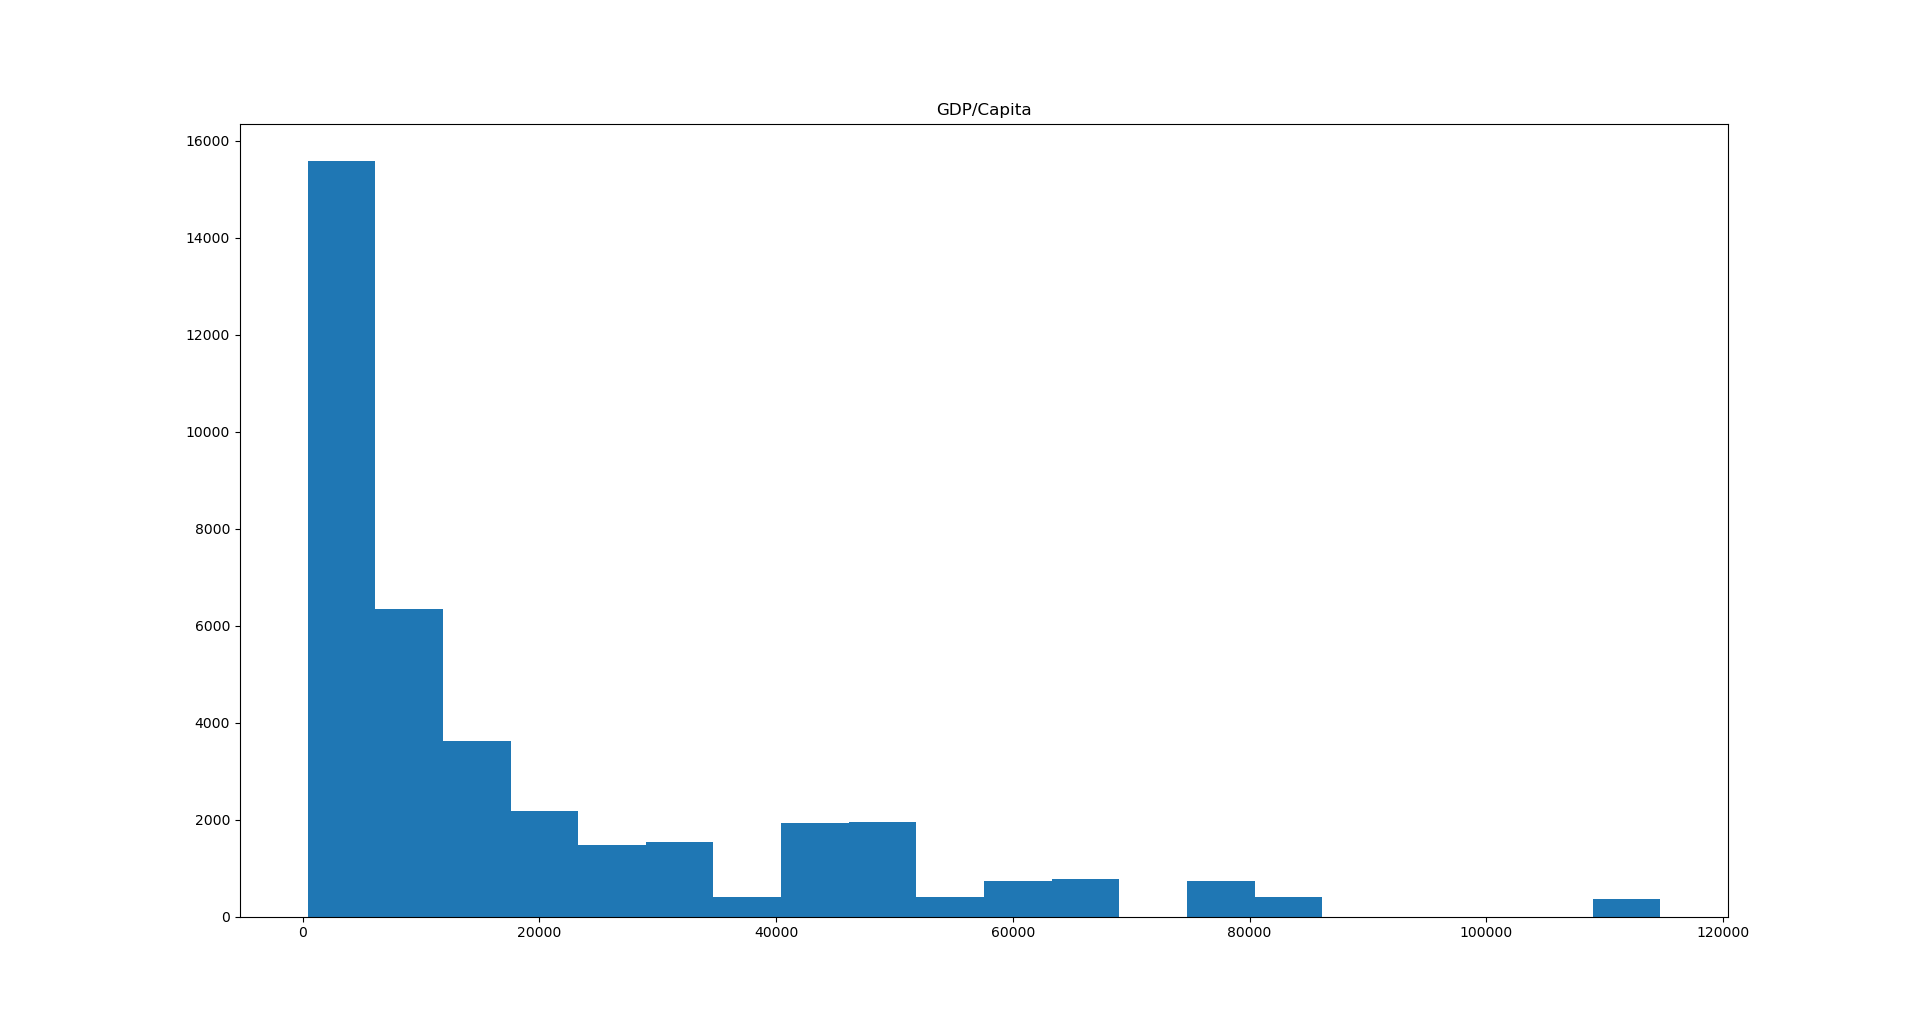
\includegraphics[width=\textwidth]{Figures/Question1/7. Histogram for GDP over capita.png}
	\caption{Ιστόγραμμα για στήλη 'GDP/Capita'}
\end{figure}

\begin{figure}[H]
	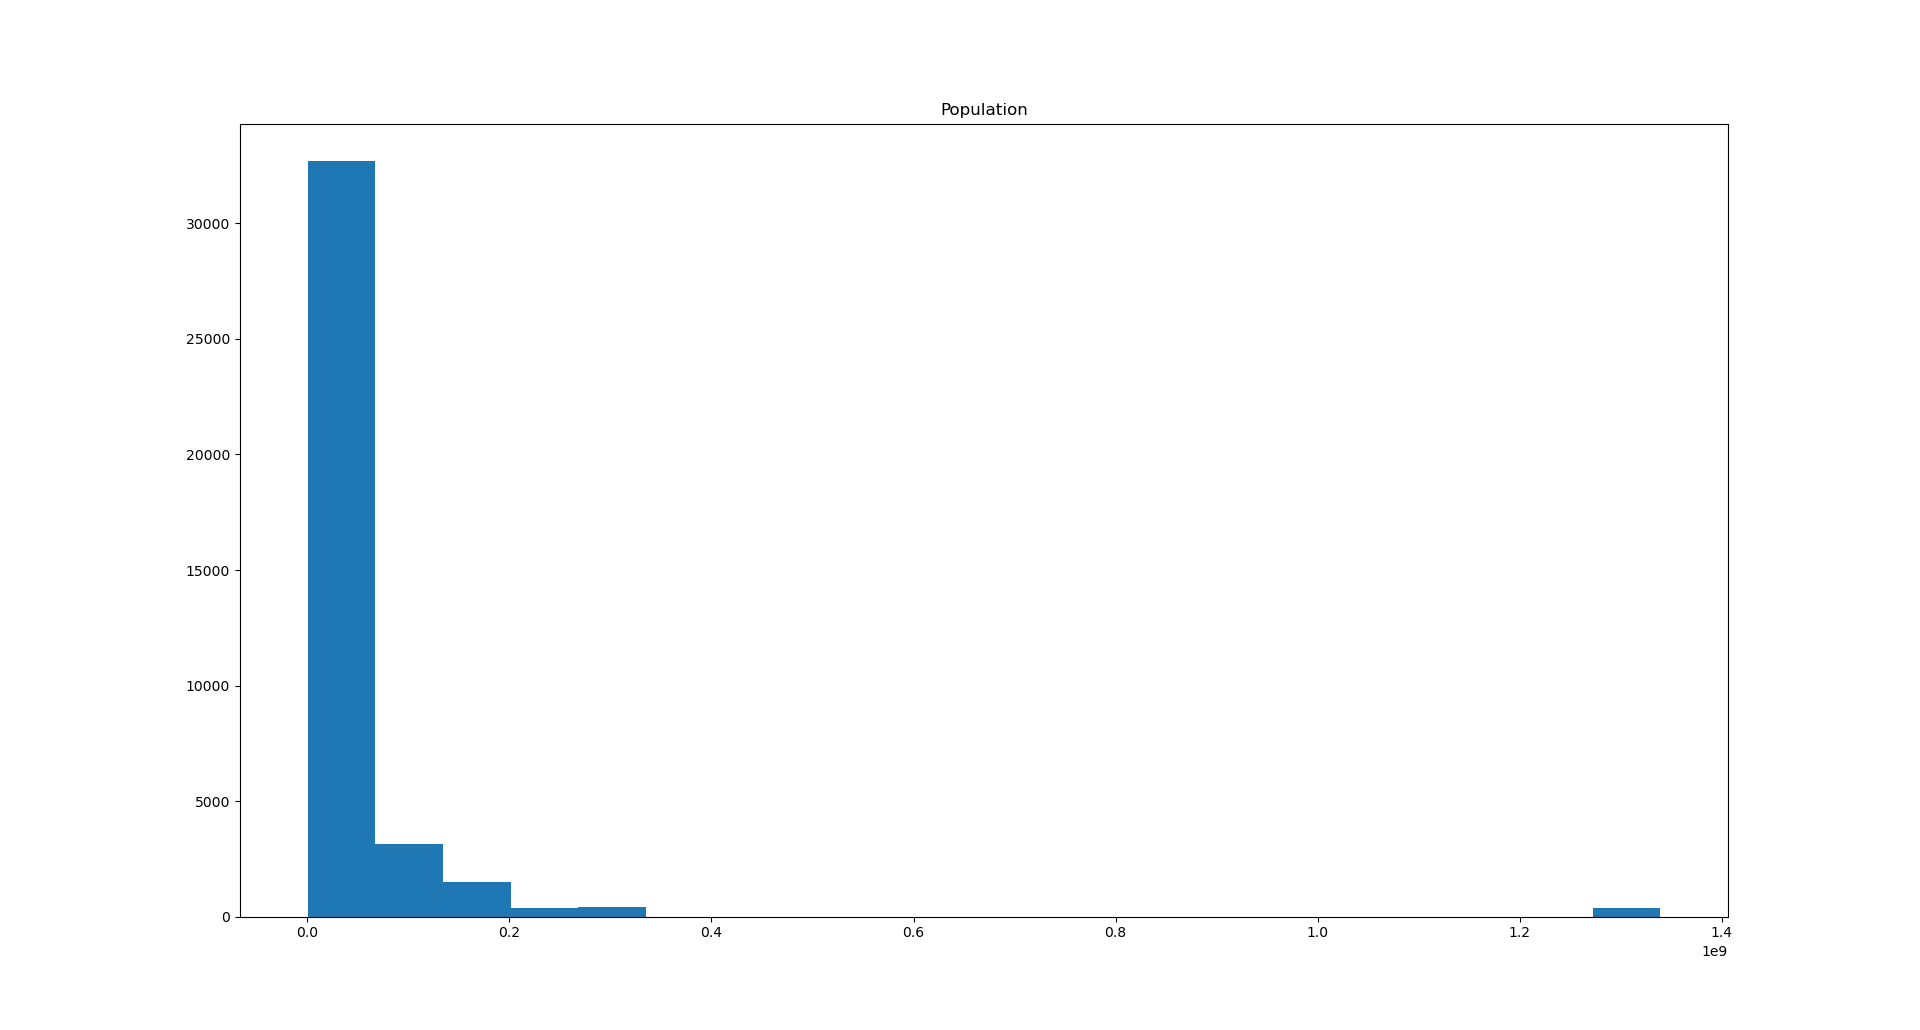
\includegraphics[width=\textwidth]{Figures/Question1/8. Histogram for population.png}
	\caption{Ιστόγραμμα για στήλη 'Population'}
\end{figure}

\begin{figure}[H]
	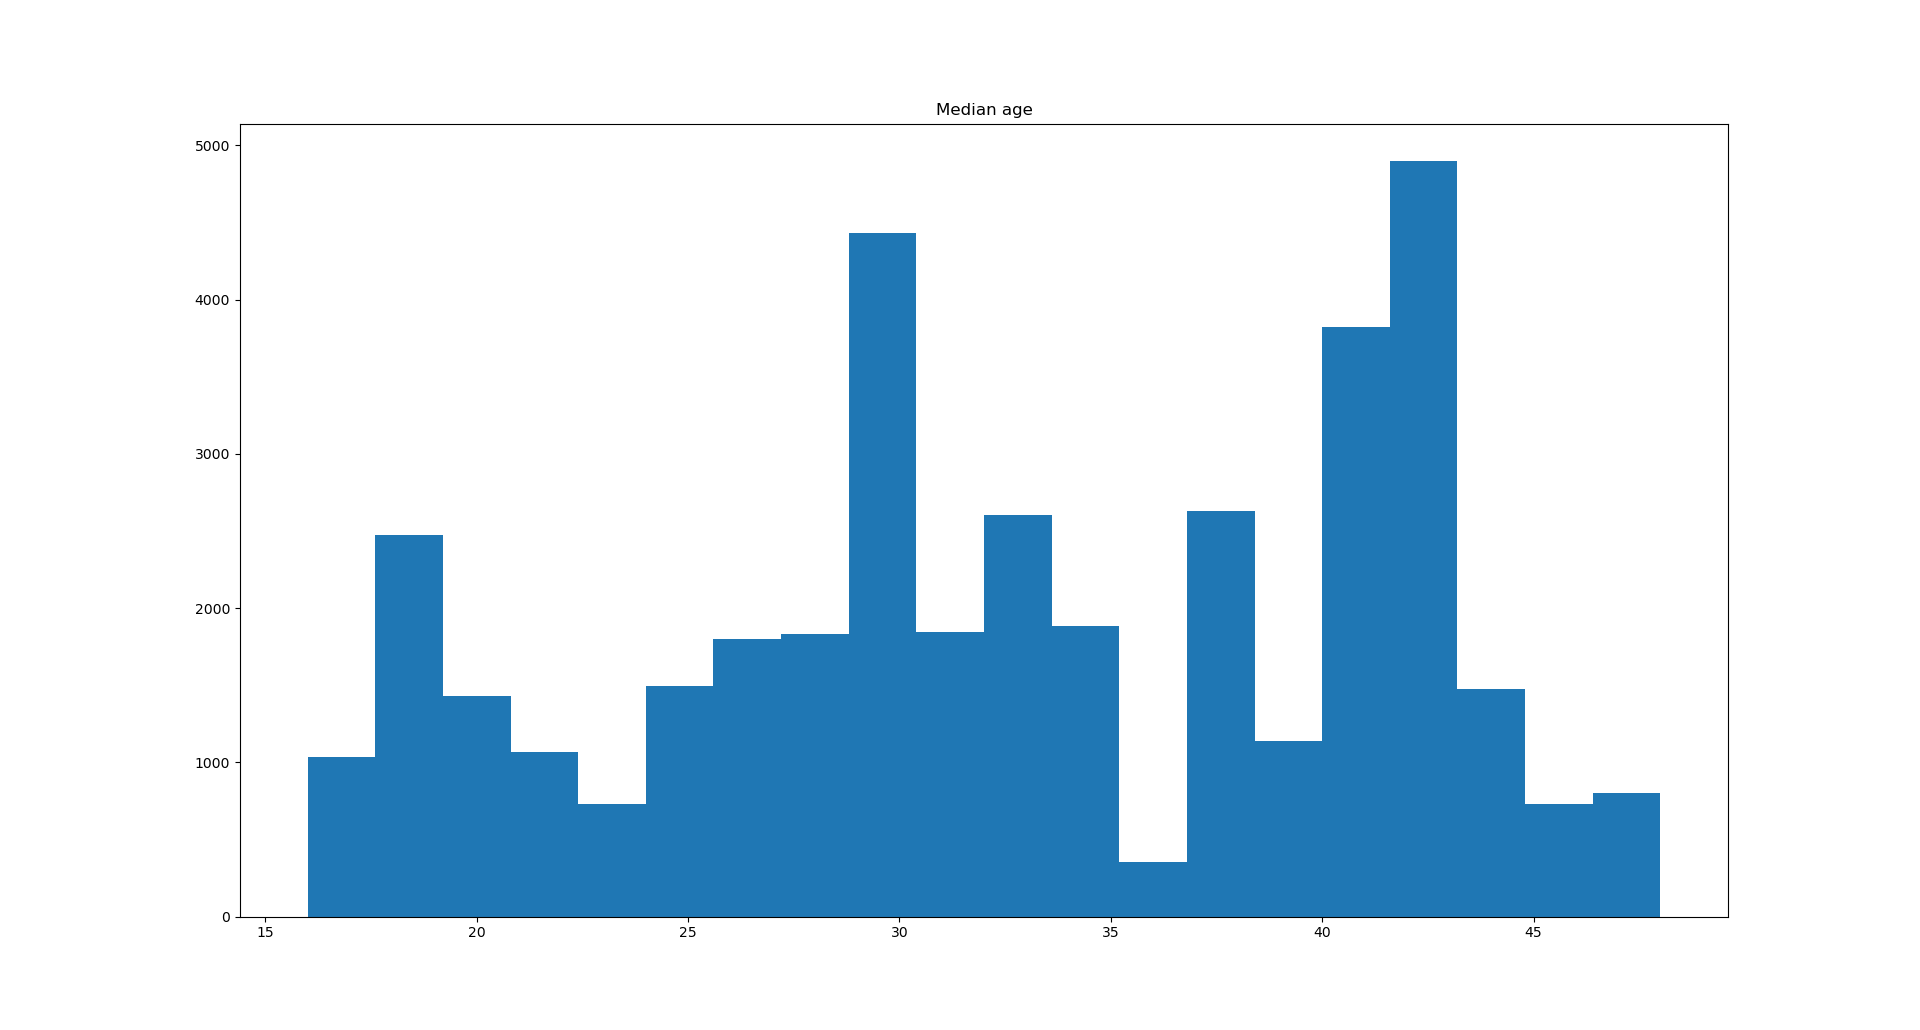
\includegraphics[width=\textwidth]{Figures/Question1/9. Histogram for median age.png}
	\caption{Ιστόγραμμα για στήλη 'Median age'}
\end{figure}

\begin{figure}[H]
	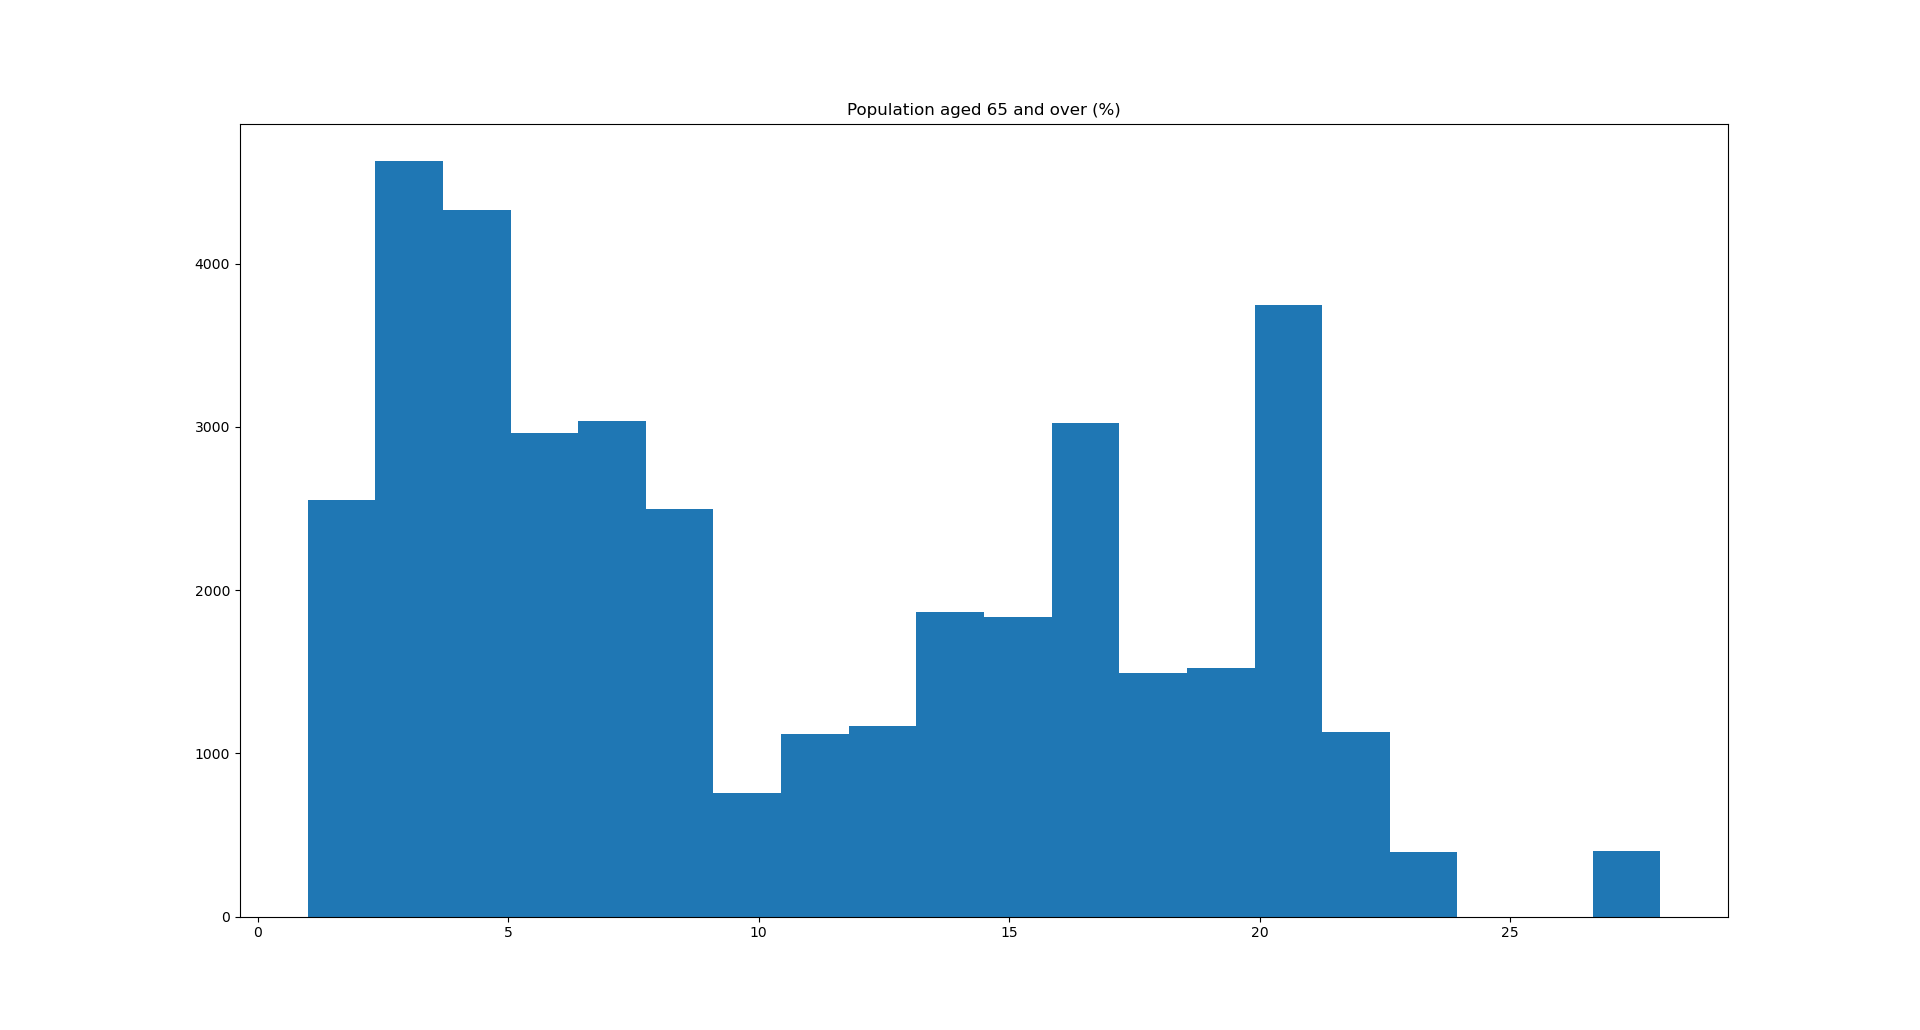
\includegraphics[width=\textwidth]{Figures/Question1/10. Histogram for population aged 65 and over.png}
	\caption{Ιστόγραμμα για στήλη 'Population aged 65 and over (\%)'}
\end{figure}

\begin{figure}[H]
	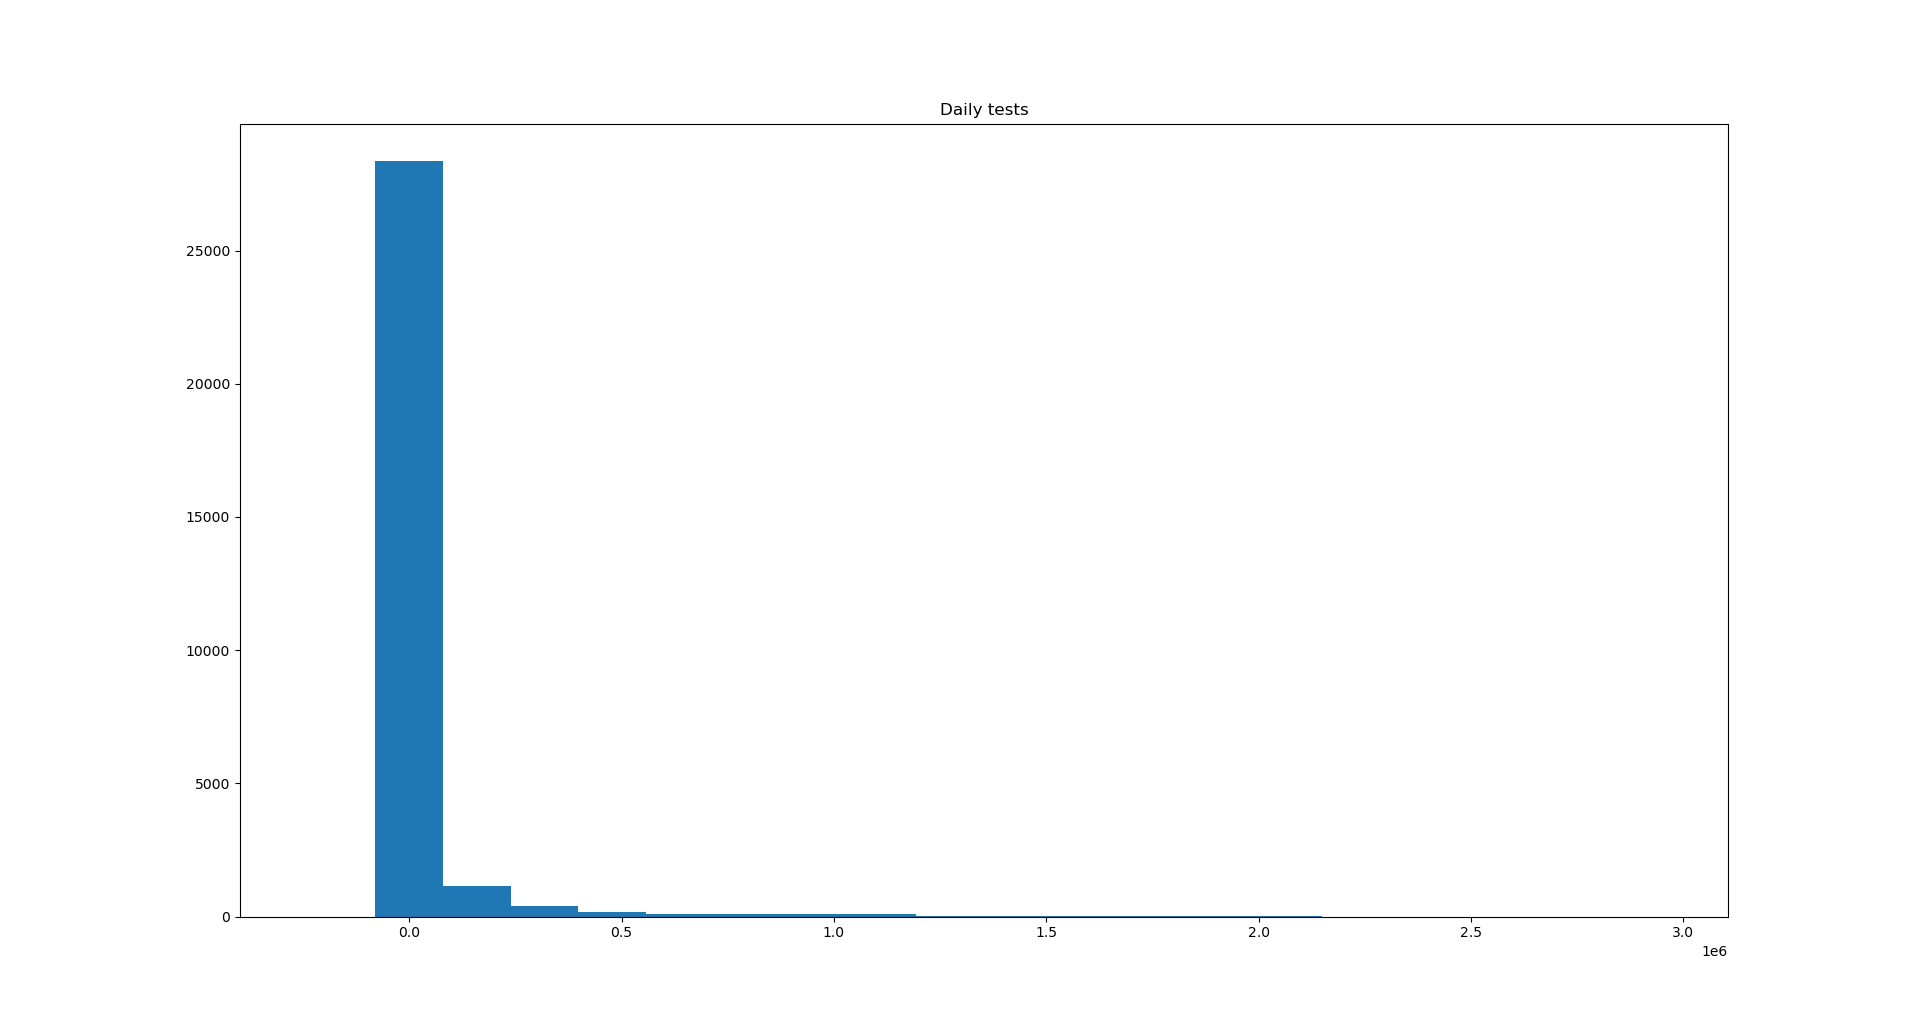
\includegraphics[width=\textwidth]{Figures/Question1/11. Histogram for daily tests.png}
	\caption{Ιστόγραμμα για στήλη 'Daily tests'}
\end{figure}

\begin{figure}[H]
	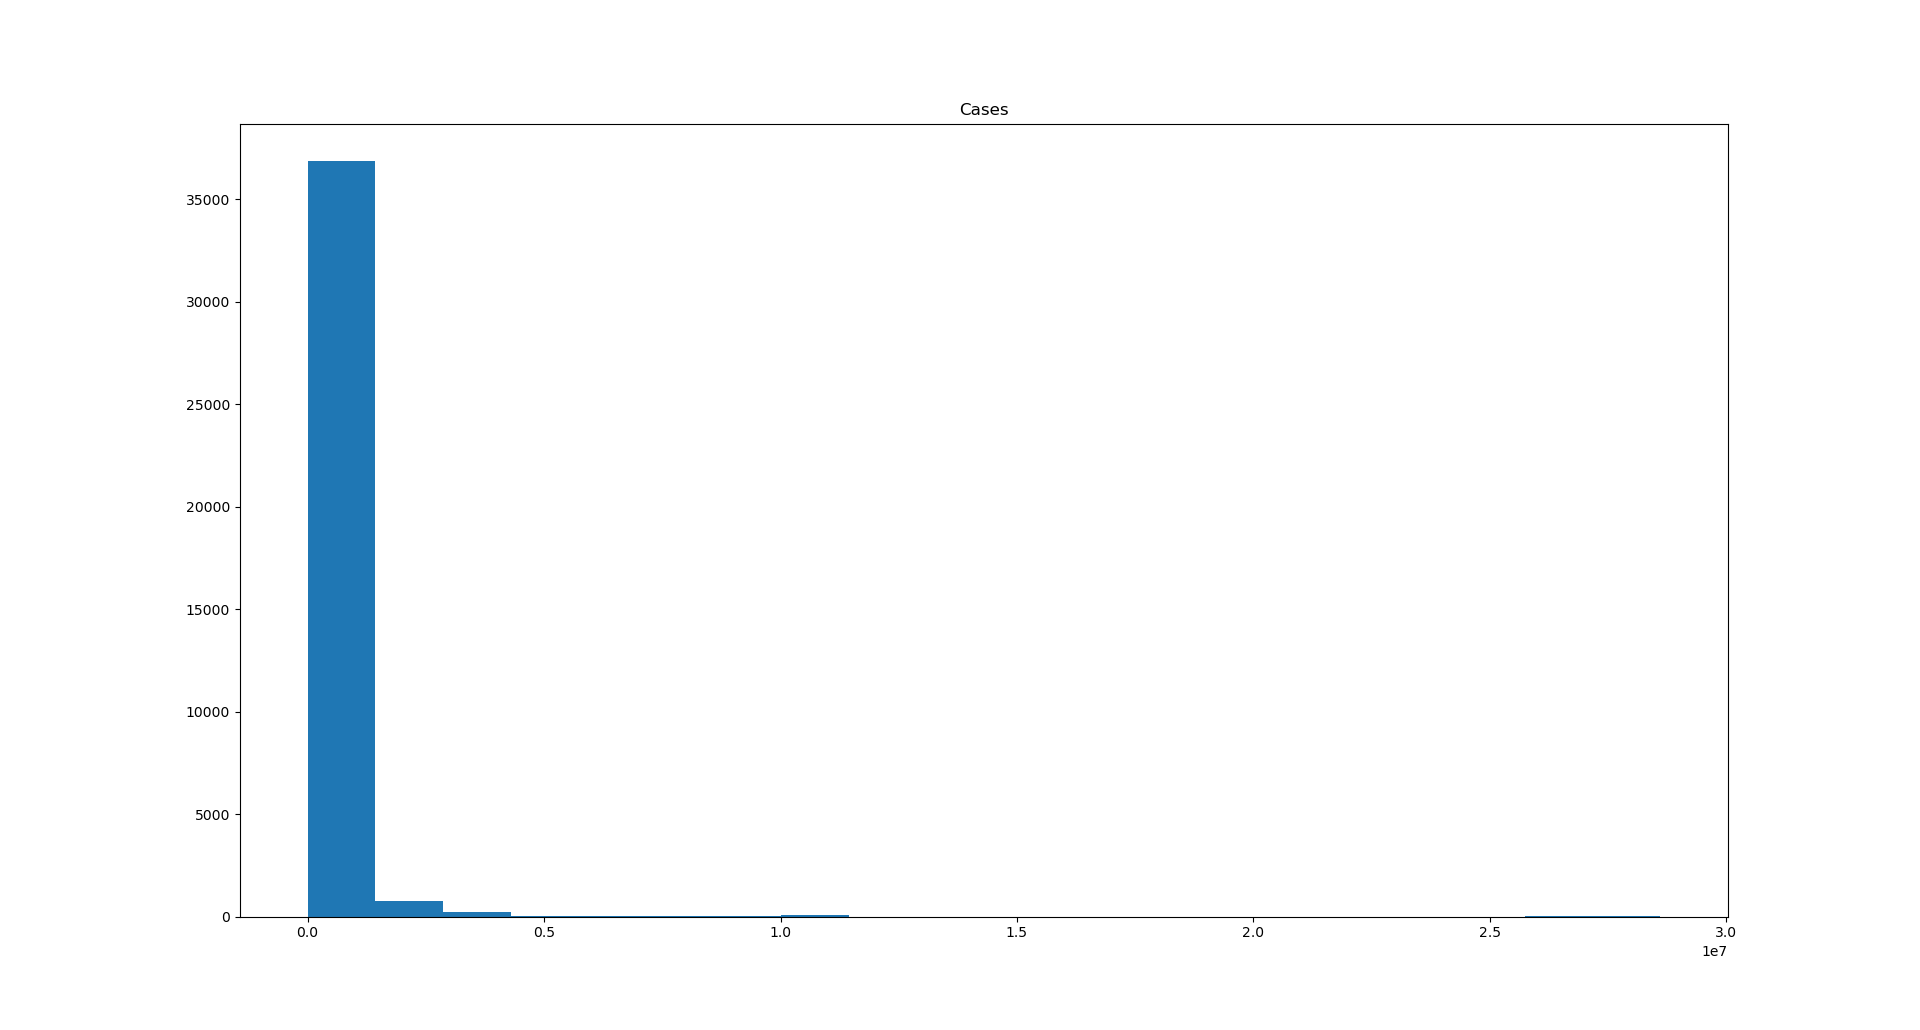
\includegraphics[width=\textwidth]{Figures/Question1/12. Histogram for cases.png}
	\caption{Ιστόγραμμα για στήλη 'Cases'}
\end{figure}

\begin{figure}[H]
	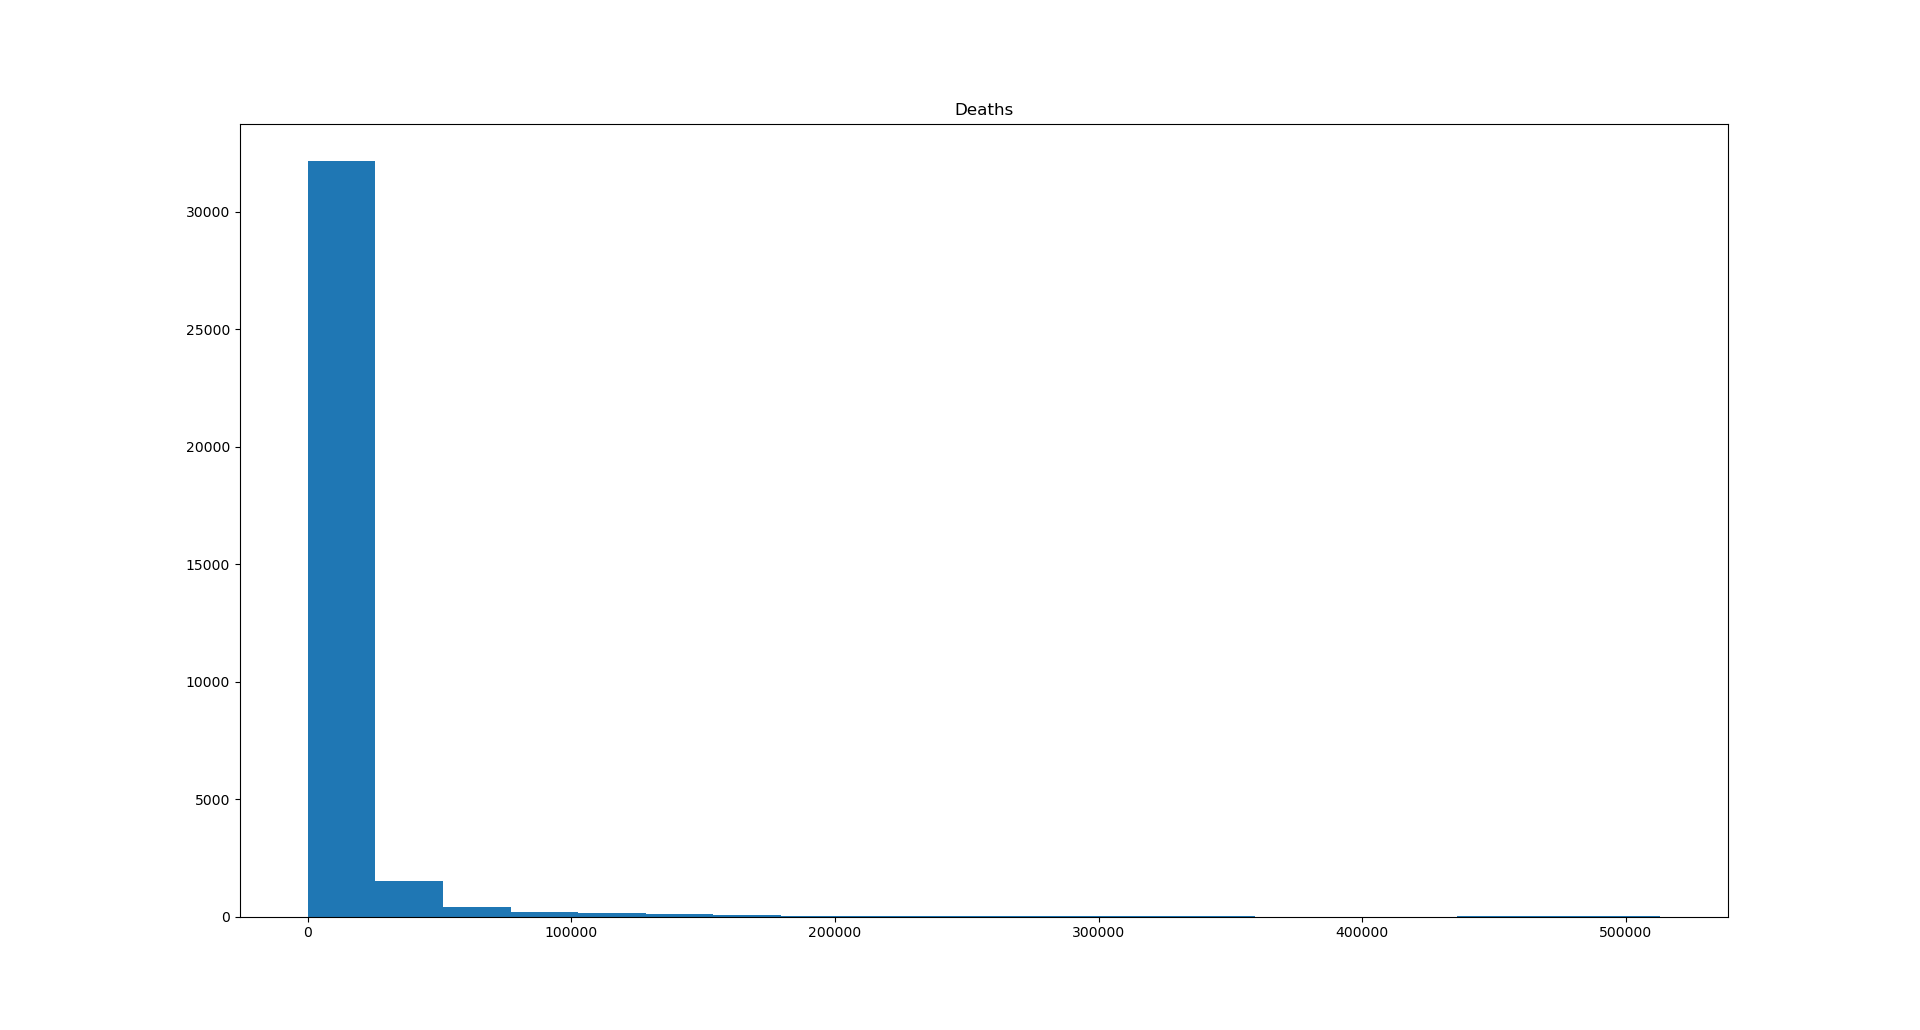
\includegraphics[width=\textwidth]{Figures/Question1/13. Histogram for deaths.png}
	\caption{Ιστόγραμμα για στήλη 'Deaths'}
\end{figure}

Τέλος παρακάτω παρουσιάζουμε το Correlation Matrix Heatmap που φτιάξαμε για τις στήλες του dataset.

\begin{figure}[H]
	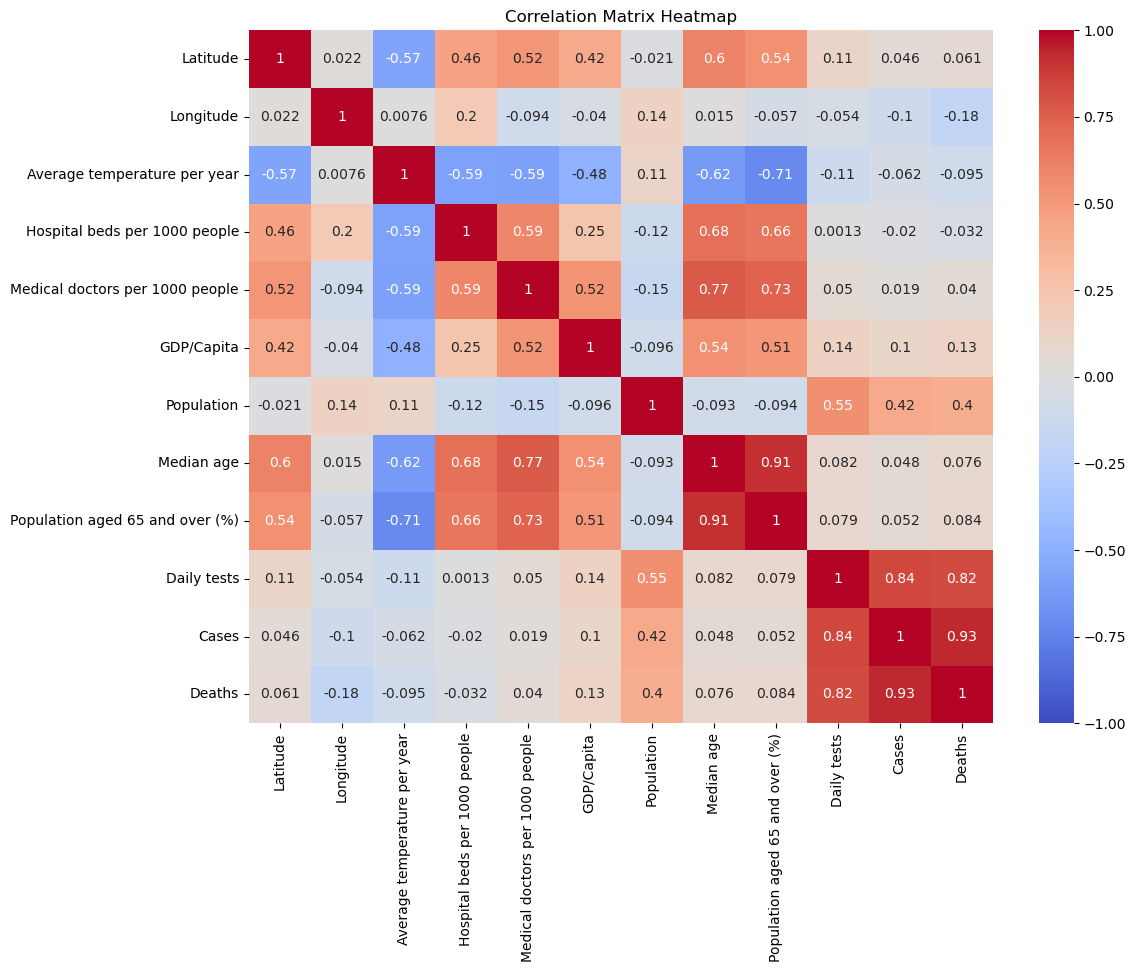
\includegraphics[width=\textwidth]{Figures/Question1/14. Correlation matrix heatmap.png}
	\caption{Correlation Matrix Heatmap για τις στήλες}
\end{figure}

\subsubsection{Συμπεράσματα}

Από τα στατιστικά στοιχεία και τα ιστογράμματα συμπεραίνουμε πως πολλές από τις στήλες περιέχουν στοιχεία που φαίνεται να αποτελούν half-normal κατανομές, με διαφορετικές τιμές μέσης τιμής και διασποράς. Οι στήλες αυτές είναι οι 'Medical doctors per 1000 people', 'GDP/Capita', 'Population', 'Daily tests', 'Cases', 'Deaths'. Επίσης η στήλη 'Hospital beds per 1000 people' φαίνεται να ακολουθεί log-normal κατανομή. Για τις υπόλοιπες στήλες δεν μπορούμε να συμπεράνουμε ότι ανήκουν σε κάποια κατανομή.

Από το Correlation Matrix Heatmap παρατηρούμε ότι υπάρχει μεγάλη συσχέτιση μεταξύ 'Daily tests', 'Cases' και 'Deaths', καθώς και μεταξύ 'Median age', 'People aged 65 and over (\%)', 'Hospital beds per 1000 people' και 'Medical doctors per 1000 people'. Υπάρχει επίσης μεγάλη αρνητική συσχέτιση μεταξύ του 'Average Temperature per year' σε σχέση με τα 'Population aged 65 and over (\%)', 'Median age', 'Medical doctors per 1000 people', 'Hospital beds per 1000 people' και 'Latitude'. Σημειώνουμε ότι υπάρχουν και άλλες συσχετίσεις εκτός από αυτές που αναφέρονται, αλλά δεν είναι τόσο ισχυρές όσο αυτές που αναφέρουμε εδώ, οπότε τις παραλείπουμε για λόγους συντομίας, εφόσον φαίνονται και στο heatmap.

\section{Υλοποίηση και Αποτελέσματα Ερωτήματος 2}

\subsection{Σύντομη Περιγραφή της Διαδικασίας Υλοποίησης}

\subsubsection{Δημιουργία Νέων Πεδίων και Επιλογή Πεδίων για το Clustering}
Αποφασίσαμε για το πιο αποτελεσματικό clustering να προσθέσουμε ορισμένα πεδία στα δεδομένα τα οποία εξάγονται από τα υπόλοιπα δεδομένα. Πιο συγκεκριμένα τα νέα πεδία αυτά τα ορίζουμε ως εξής:

\begin{itemize}
    \item Positive Ratio = Today's New Cases / Daily Tests
    \item Death Ratio = Total Deaths / Total Cases
    \item Tested Ratio = Daily Tests / Population
\end{itemize}

Αποφασίσαμε επίσης να χρησιμοποιήσουμε τα πεδία 'Cases', 'Deaths', 'Positive Ratio', 'Death Ratio' και 'Tested Ratio' για το clustering που θα κάνουμε, επειδή πιστεύουμε πως αυτές οι μετρικές είναι που περιέχουν τη πληροφορία της απόδοσης κάθε χώρας στην αντιμετώπιση του ιού.

Ο λόγος που συμπεριλαμβάνουμε τα 'Cases' και 'Deaths' ενώ έχουμε ήδη τα 'Positive Ratio' και 'Deaths Ratio' είναι επειδή θεωρούμε πως μια χώρα που έχει πολλά κρούσματα και θανάτους θα μπορούσε να έχει αντίστοιχα και μικρά ratio, αν είχε αρκετά μεγάλο πληθυσμό και μεγάλο αριθμό καθημερινών τεστ, αλλά η ανθρώπινη απώλεια παραμένει μεγάλη και ας είναι τα ποσοστά μικρά.

Επίσης σημειώνουμε ότι θα κάνουμε aggregate τα δεδομένα όλων των ημερών, οπότε πεδία όπως το 'Date' δεν μας χρειάζονται, όπως θα εξηγηθεί σε παρακάτω υποενότητα.

\subsubsection{Χειρισμός Τιμών που Λείπουν}

Για την υλοποίηση του ερωτήματος αυτού, αρχικά αφού διαβάσουμε το αρχείο του dataset θα πρέπει να αντιμετωπίσουμε τις τιμές που λείπουν από αυτό. Αυτό το επιτυγχάνουμε με τη χρήση των εντολών:

\begin{lstlisting}[language=Python]
df = df.groupby('Entity',group_keys=False).apply(lambda x: x.fillna(method='ffill'))
df = df.groupby('Entity',group_keys=False).apply(lambda x: x.fillna(method='bfill'))
\end{lstlisting}

Αυτές οι εντολές επιτυγχάνουν αρχικά το grouping του DataFrame με βάση το 'Entity' (χώρα) και μετά την εφαρμογή της fillna μεθόδου, η οποία συμπληρώνει τις τιμές που λείπουν αρχικά με χρήση forward fill στη πρώτη εντολή και έπειτα με backward fill στη δεύτερη εντολή.

Το forward fill επιτυγχάνει την αντικατάσταση τιμών που λείπουν με την τελευταία προηγούμενη καταγεγραμμένη τιμή, αλλά επειδή γίνεται να υπάρχουν ακόμα κενά (πχ αν λείπουν τιμές στην αρχή των καταγεγραμμένων στοιχείων), κάνουμε έπειτα το backward fill που συμπληρώνει τιμές που λείπουν με την επόμενη καταγεγραμμένη τιμή.

Ο λόγος που προτιμούμε πρώτα να κάνουμε forward fill και μετά backward fill είναι επειδή με αυτόν τον τρόπο ελαχιστοποιούμε την συμπλήρωση με βάση τις μελλοντικές ως προς τη χρονική στιγμή που συμπληρώνουμε τιμές.

Έπειτα αφαιρούμε όλα τα duplicates που τυχόν προέκυψαν με χρήση της μεθόδου drop\_duplicates() του Pandas.

\subsubsection{Προεπεξεργασία Δεδομένων}

Το πρώτο βήμα της προεπεξεργασίας θα είναι να κάνουμε aggregation των δεδομένων. Έτσι αντί να αποθηκεύουμε για κάθε χώρα τα δεδομένα κάθε μέρας ξεχωριστά, θα αποθηκεύσουμε είτε τον μέσο όρο είτε την τελευταία τιμή μιας στήλης δεδομένων κάθε φορά. Αυτό μας διευκολύνει στο clustering, επειδή μειώνει τον όγκο των δεδομένων εισόδου και ταυτόχρονα απομονώνει την σημαντική πληροφορία από τα δεδομένα για όλες τις ημέρες. Σημειώνουμε επίσης ότι κάνουμε aggregation σε όλα τα δεδομένα, με σκοπό να τυπώσουμε στατιστικά για τα clusters με βάση όλα τα πεδία δεδομένων.

Έτσι θα αποθηκεύσουμε τη μέση τιμή των 'Positive Ratio', 'Death Ratio', και 'Tested Ratio' και θα αποθηκεύσουμε και την τελευταία τιμή που εμφανίζεται για όλα τα υπόλοιπα Series.

Επειδή το 'Continent' περιέχει κατηγορικά δεδομένα, αποφασίζουμε να τα μετατρέψουμε σε αριθμητικά δεδομένα ώστε να μπορέσουμε να κάνουμε κανονικοποίηση αργότερα πάνω σε αυτά. Άρα κάνουμε one-hot encoding για όλο το Series 'Continent' πάνω στο DataFrame που προέκυψε από το προηγούμενο βήμα.

Έπειτα αφαιρούμε το Series 'Date' από το DataFrame των προηγούμενων βημάτων, επειδή αυτό είναι ίδιο σε κάθε περίπτωση (ίσο με την τελευταία ημερομηνία του dataset).

Τέλος κάνουμε κανονικοποίηση στα δεδομένα (με χρήση αντικειμένου StandardScaler της βιβλιοθήκης Scikit-learn) και αποθηκεύουμε τα τελικά δεδομένα στη μεταβλητή \\normalized\_data.

\subsubsection{Δημιουργία Δενδρογράμματος και Συσταδοποίηση}

Αρχικά σημειώνουμε πως για την συσταδοποίηση αποφασίσαμε να χρησιμοποιήσουμε agglomerative clustering, επειδή στις δοκιμές μας εμφάνισε τα καλύτερα αποτελέσματα.

Πριν την συσταδοποίηση όμως είναι σημαντικό να προσεγγίσουμε τον ιδανικό αριθμό των clusters στον οποίο θα χωρίσουμε τις χώρες. Με σκοπό να το επιτύχουμε αυτό δημιουργούμε την τεχνική του δενδρογράμματος, οπότε αρχικά φτιάχνουμε το δενδρόγραμμα χρησιμοποιώντας τις εντολές dendgrogram() και linkage() της βιβλιοθήκης SciPy. Από το δενδρόγραμμα αυτό, μπορούμε έπειτα να προσεγγίσουμε τον ιδανικό αριθμό clusters, παίρνοντας το μέσο της μεγαλύτερης απόστασης μεταξύ διαδοχικών clusterings, τραβώντας οριζόντια ευθεία που περνάει από αυτό το σημείο, και βλέποντας πόσες κάθετες ευθείες τέμνονται από την νέα ευθεία, το οποίο είναι η προσέγγιση του αριθμού των clusters που θέλουμε. Την ευθεία αυτή που προέκυψε την σχεδιάζουμε πάνω στο γράφημα για διευκόλυνση εντοπισμού της.

Έπειτα με σκοπό την επίτευξη του agglomerative clustering, χρησιμοποιούμε την συνάρτηση AgglomerativeClustering() της βιβλιοθήκης Scikit-learn, επιλέγοντας αριθμό clusters με βάση το παραπάνω κριτήριο (θα δείξουμε τον αριθμό που επιλέξαμε παρακάτω στα αποτελέσματα).

Σημειώνουμε επίσης εδώ πως ως τεχνική linkage για τον σχεδιασμό του δενδρογράμματος και για το clustering χρησιμοποιήσαμε Ward, επειδή με αυτό μετά από δοκιμές κρίναμε ότι επιτύχαμε τα καλύτερα αποτελέσματα.

Τέλος τυπώνουμε τα clusters που προέκυψαν μαζί με τιμές μέσης τιμής και διακύμανσης για όλα τα πεδία δεδομένων με βάση το περιεχόμενο χωρών του κάθε cluster.

\subsection{Τελικά Αποτελέσματα και Σχολιασμός τους}

\subsubsection{Αποτελέσματα Δενδρογράμματος}

Παρακάτω παρουσιάζουμε τον δενδρόγραμμα που προέκυψε από την εκτέλεση του κώδικα:

\begin{figure}[H]
	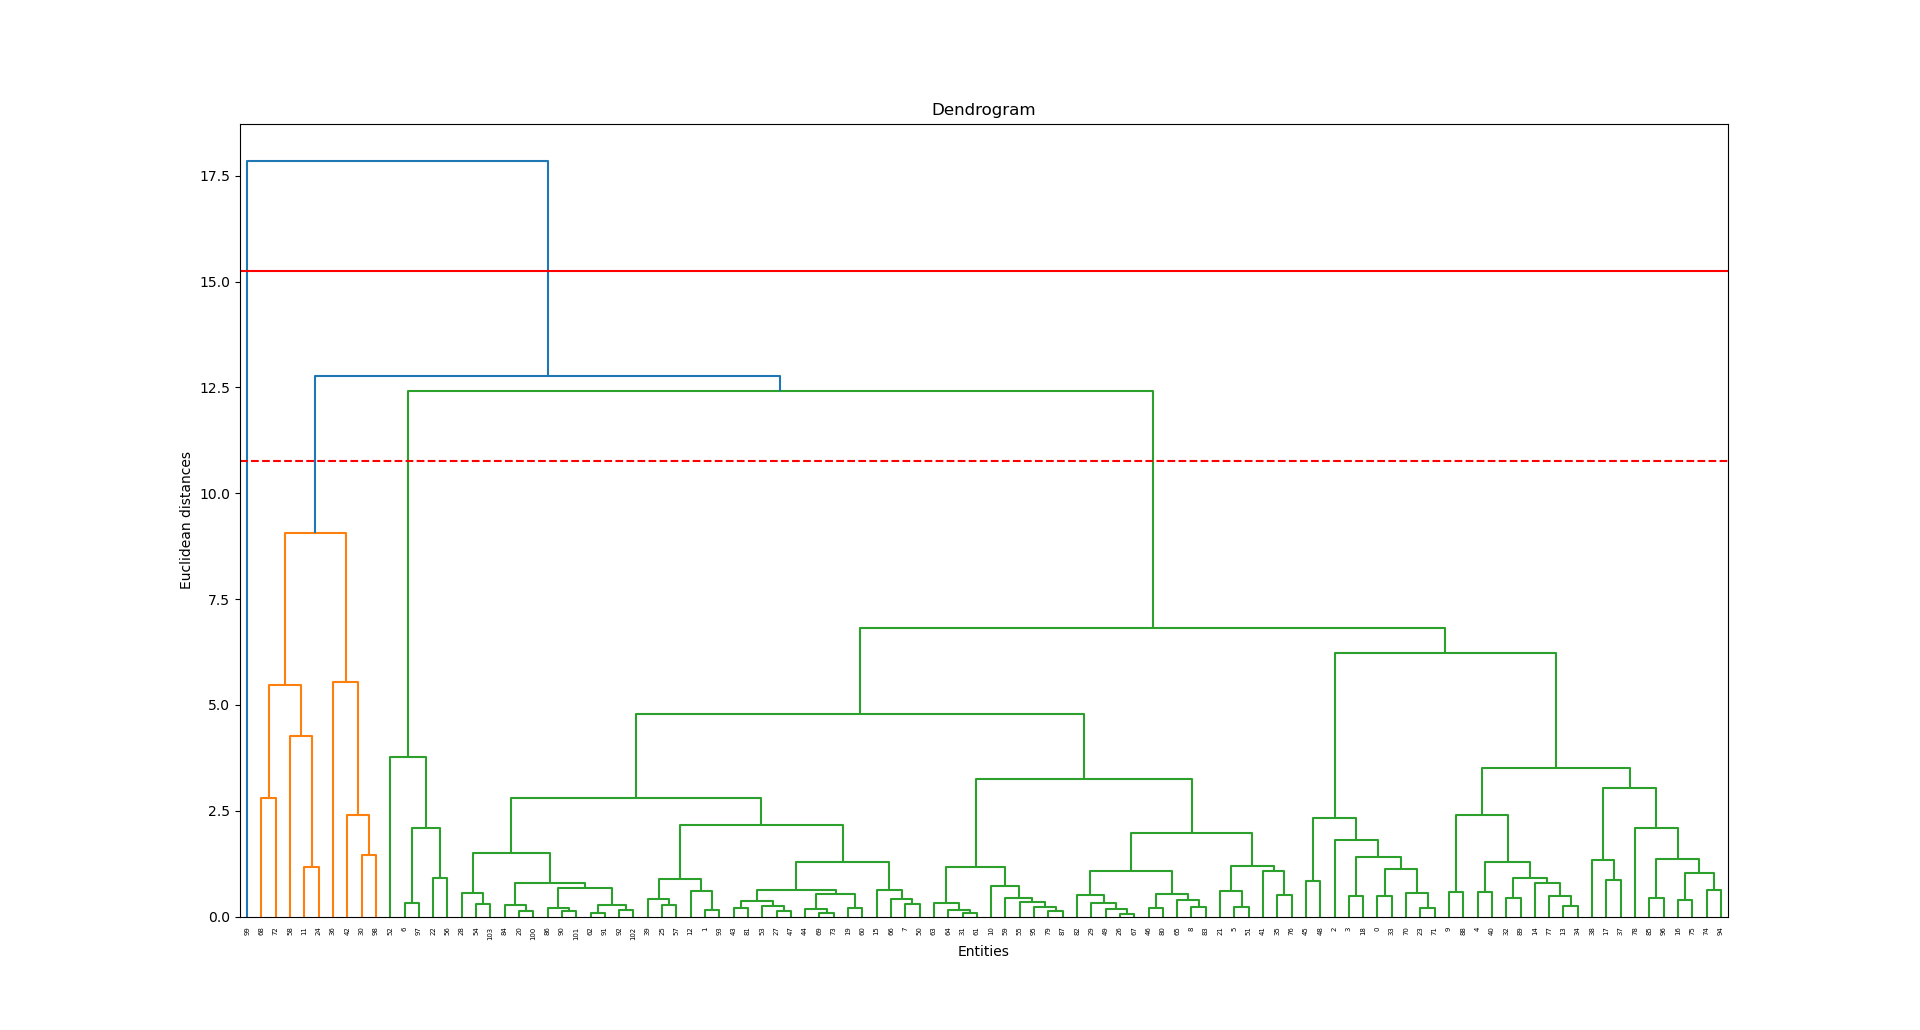
\includegraphics[width=\textwidth]{Figures/Question2/1. Dendrogram.png}
	\caption{Δενδρόγραμμα για προσέγγιση αριθμού clusters στο Agglomerative Clustering}
\end{figure}

Παρατηρούμε ότι το μέση της μεγαλύτερης απόστασης μεταξύ groupings γίνεται εκεί που έχουμε σχεδιάσει την κόκκινη συνεχή γραμμή. Οπότε η γραμμή αυτή τέμνει 2 κάθετες γραμμές, οπότε η προσέγγιση του ιδανικού αριθμού clusters που κάναμε οδήγησε σε 2 clusters.

Επειδή όμως παρατηρούμε πως με 2 clusters, ο διαχωρισμός που γίνεται είναι η Ηνωμένες Πολιτείες σε ένα cluster και όλες οι υπόλοιπες χώρες στο άλλο, αποφασίσαμε να προτιμήσουμε μεγαλύτερο αριθμό cluster για να γίνει καλύτερος διαχωρισμός και των υπόλοιπων χωρών.

Άρα πήραμε και το μέσο της δεύτερης μεγαλύτερης απόστασης μεταξύ groupings, το οποίο βρίσκεται εκεί που σχεδιάσαμε τη κόκκινη διακεκομμένη γραμμή, η οποία τέμνει συνολικά 4 κάθετες γραμμές, οπότε θα πάρουμε τελικά 4 clusters.

\subsubsection{Αποτελέσματα Agglomerative Clustering με 3 Clusters}

Άρα προχωρώντας τώρα στη διαδικασία του agglomerative clustering με συνολικό αριθμό 4 clusters, δημιουργούνται τα εξής clusters:

\begin{itemize}
    \item \textbf{Cluster 1:} Bolivia, Ecuador, France, India, Italy, Mexico, Oman, Peru, United Kingdom
    \item \textbf{Cluster 2:} Bahrain, Denmark, Luxembourg, Malta, United Arab Emirates
    \item \textbf{Cluster 3:} Albania, Algeria, Argentina, Armenia, Australia, Austria, Bangladesh, Belarus, Belgium, Bhutan, Bosnia and Herzegovina, Bulgaria, Canada, Cape Verde, Chile, Colombia, Costa Rica, Croatia, Cuba, Cyprus, Dominican Republic, El Salvador, Estonia, Ethiopia, Fiji, Finland, Ghana, Greece, Guatemala, Hungary, Iceland, Indonesia, Iran, Iraq, Ireland, Israel, Jamaica, Japan, Jordan, Kazakhstan, Kenya, Kuwait, Latvia, Libya, Lithuania, Madagascar, Malawi, Malaysia, Mauritania, Mongolia, Morocco, Mozambique, Myanmar, Namibia, Nepal, New Zealand, Nigeria, Norway, Pakistan, Panama, Paraguay, Philippines, Poland, Portugal, Qatar, Romania, Russia, Rwanda, Saudi Arabia, Senegal, Serbia, Slovakia, Slovenia, South Africa, South Korea, Sri Lanka, Sweden, Switzerland, Thailand, Togo, Trinidad and Tobago, Tunisia, Turkey, Uganda, Ukraine, Uruguay, Vietnam, Zambia, Zimbabwe
    \item \textbf{Cluster 4:} United States
\end{itemize}

Τα παραπάνω clusters έχουν τα εξής στατιστικά στοιχεία:

\begin{itemize}
    \item \textbf{Cluster 1:}
        \begin{itemize}
            \item \textbf{Continent}: mean = 3.11, std = 1.90
            \item \textbf{Latitude}: mean = 20.21, std = 25.20
            \item \textbf{Longitude}: mean = -19.24, std = 63.74
            \item \textbf{Average temperature per year}: mean = 19.00, std = 6.30
            \item \textbf{Hospital beds per 1000 people}: mean = 2.16, std = 1.63
            \item \textbf{GDP/Capita}: mean = 17794.94, std = 16294.37
            \item \textbf{Population}: mean = 191834882.78, std = 431981760.13
            \item \textbf{Median age}: mean = 33.11, std = 7.75
            \item \textbf{Cases}: mean = 2895673.11, std = 3435746.96
            \item \textbf{Deaths}: mean = 80524.89, std = 66528.05
            \item \textbf{Positive Ratio}: mean = 24.19, std = 21.13
            \item \textbf{Death Ratio}: mean = 5.70, std = 3.28
            \item \textbf{Tested Ratio}: mean = 0.07, std = 0.08
        \end{itemize}
    \item \textbf{Cluster 2:}
        \begin{itemize}
            \item \textbf{Continent}: mean = 2.60, std = 2.19
            \item \textbf{Latitude}: mean = 38.27, std = 14.45
            \item \textbf{Longitude}: mean = 26.90, std = 23.35
            \item \textbf{Average temperature per year}: mean = 18.40, std = 9.79
            \item \textbf{Hospital beds per 1000 people}: mean = 2.94, std = 1.50
            \item \textbf{GDP/Capita}: mean = 54260.56, std = 36592.93
            \item \textbf{Population}: mean = 3545414.60, std = 3924438.31
            \item \textbf{Median age}: mean = 37.80, std = 4.60
            \item \textbf{Cases}: mean = 160678.60, std = 148003.57
            \item \textbf{Deaths}: mean = 996.80, std = 837.92
            \item \textbf{Positive Ratio}: mean = 1.58, std = 0.91
            \item \textbf{Death Ratio}: mean = 1.17, std = 0.77
            \item \textbf{Tested Ratio}: mean = 0.66, std = 0.22
        \end{itemize}
    \item \textbf{Cluster 3:} 
        \begin{itemize}
            \item \textbf{Continent}: mean = 3.03, std = 1.87
            \item \textbf{Latitude}: mean = 22.72, std = 26.86
            \item \textbf{Longitude}: mean = 24.57, std = 60.09
            \item \textbf{Average temperature per year}: mean = 17.73, std = 8.29
            \item \textbf{Hospital beds per 1000 people}: mean = 3.25, std = 2.67
            \item \textbf{GDP/Capita}: mean = 16131.40, std = 19720.59
            \item \textbf{Population}: mean = 31919538.49, std = 48260254.66
            \item \textbf{Median age}: mean = 32.16, std = 8.79
            \item \textbf{Cases}: mean = 418219.00, std = 667666.16
            \item \textbf{Deaths}: mean = 8966.71, std = 15522.94
            \item \textbf{Positive Ratio}: mean = 6.48, std = 6.16
            \item \textbf{Death Ratio}: mean = 2.12, std = 1.20
            \item \textbf{Tested Ratio}: mean = 0.07, std = 0.07
        \end{itemize}
    \item \textbf{Cluster 3:} 
        \begin{itemize}
            \item \textbf{Continent}: mean = 6.00, std = nan
            \item \textbf{Latitude}: mean = 37.09, std = nan
            \item \textbf{Longitude}: mean = -95.71, std = nan
            \item \textbf{Average temperature per year}: mean = 11.00, std = nan
            \item \textbf{Hospital beds per 1000 people}: mean = 2.77, std = nan
            \item \textbf{GDP/Capita}: mean = 65297.50, std = nan
            \item \textbf{Population}: mean = 325719178.00, std = nan
            \item \textbf{Median age}: mean = 38.00, std = nan
            \item \textbf{Cases}: mean = 28605669.00, std = nan
            \item \textbf{Deaths}: mean = 513091.00, std = nan
            \item \textbf{Positive Ratio}: mean = 6.76, std = nan
            \item \textbf{Death Ratio}: mean = 3.05, std = nan
            \item \textbf{Tested Ratio}: mean = 0.24, std = nan

        \end{itemize}
\end{itemize}

\subsubsection{Συμπεράσματα}

Παρατηρώντας τα αποτελέσματα της συσταδοποίησης παρατηρούμε ότι η πρώτη συστάδα περιείχε χώρες με σχετικά κακή αντιμετώπιση του ιού, που ξεχώριζαν για το μεγάλο 'Positive Ratio' (= 24.19\%) που είχαν καθώς και για το συγκριτικά μεγάλο 'Death Ratio' (= 5.7\%) και μικρό 'Tested Ratio' (= 0.07\&) που είχαν. Άρα αυτές αποτελούν χώρες που έκαναν τεστ μόνο σε άτομα που είχαν μεγάλη πιθανότητα να έχουν κολλήσει, το οποίο υπάρχει πιθανότατα, λόγω της έλλειψης πρόληψης, να συνέβαλλε και στους αυξημένους θανάτους.

Στη δεύτερη συστάδα βρίσκονται οι χώρες που είχαν εξαιρετική αντιμετώπιση του ιού, το οποίο φαίνεται από τις χαμηλές συγκριτικά με τις άλλες συστάδες τιμές του 'Death Ratio' (= 1.17\%), Positive Ratio (= 1.58\%), 'Deaths' (= 996.8) και 'Cases' (= 160678).

Στη τρίτη συστάδα βρίσκονται οι χώρες που είχαν μέτρια αντιμετώπιση του ιού, που χαρακτηρίζεται από τις τιμές του 'Cases' (= 418219), 'Deaths' (= 8966.71), 'Positive Ratio' (= 6.48), 'Death Ratio' (= 2.12) οι οποίες είναι μικρότερες από αυτές της συστάδας 1 και 4, αλλά ταυτόχρονα μεγαλύτερες της συστάδας 2.

Τέλος στη τέταρτη συστάδα βρίσκονται οι Ηνωμένες Πολιτείες μόνο, που για αυτό το λόγο θεωρούμε πως ήταν outlier, η οποία είχε τιμές περίπου αντίστοιχες της συστάδας 3 για το 'Positive Ratio', 'Death Ratio' και 'Tested Ratio', αλλά ξεχώριζε κυρίως για την ιδιαίτερα μεγάλη τιμή των 'Cases' (= 28605669) και τον ιδιαίτερα μεγάλο αριθμό των 'Deaths' (= 513091). Οπότε θεωρούμε πως είχε από τις χειρότερες επιδόσεις, και ας είναι τα ποσοστά σχετικά μικρά.

Άρα συμπεραίνουμε πως οι χώρες που ξεχώρισαν αρνητικά είναι αυτές της συστάδας 1 και 4 και αυτές που ξεχώρισαν θετικά είναι αυτές της συστάδας 2. Οι χώρες αυτές μοιράζονται χαρακτηριστικά, που δεν έχουν όμως να κάνουν με την επίδοση της χώρας στην αντιμετώπιση του ιού, όπως το 'Average temperature per year' (συστάδες 1 και 2), 'Hospital beds per 1000 people', 'GDP/Capita' και 'Median Age' (συστάδες 2 και 4).

Σημειώνουμε πως πολλές από αυτές τις τιμές, όπως το 'Hospital beds per 1000 people' και το 'GDP/Capita' και 'Median Age' θα μπορούσαν να επηρεάσουν έμμεσα τη επίδοση της χώρας στην αντιμετώπιση του ιού, αλλά αυτό θα είχε ήδη αποτυπωθεί στις 5 μετρικές που χρησιμοποιήσαμε για το clustering ('Cases', 'Deaths', Positive Ratio', 'Death Ratio', και 'Tested Ratio'), οπότε θεωρούμε πως άλλοι πιο ισχυροί παράγοντες από αυτούς που αναφέρθηκαν δημιούργησαν τη διαφοροποίηση στην απόδοση μεταξύ των συστάδων.

\textbf{Σημείωση:} Εκτός από την προσέγγιση του agglomerative clustering με 3 clusters που αναφέρθηκε παραπάνω έχουμε δοκιμάσει και άλλες διαφορετικές προσεγγίσεις clustering, όπως με kmeans, χρησιμοποιώντας όλα τα πεδία δεδομένων και με διαφορετικούς αριθμούς clusters. Παρατηρήσαμε όμως πως η προσέγγιση που εξηγήσαμε παραπάνω παρουσίαζε τα καλύτερα αποτελέσματα οπότε δεν εξηγήσαμε τις άλλες, παρόλα αυτά παρέχονται και οι προσεγγίσεις αυτές σε μορφή κώδικα στο GitHub στον φάκελο 'Code/Extras - Different Tested Approaches'.

\section{Υλοποίηση και Αποτελέσματα Ερωτήματος 3}

\subsection{Σύντομη Περιγραφή της Διαδικασίας Υλοποίησης}

\subsubsection{Απομόνωση και Προεπεξεργασία Δεδομένων}

Αρχικά δημιουργούμε νέο DataFrame, το 'greece\_df' που περιέχει τα πεδία 'Date', 'Cases' και 'Daily tests' από τα δεδομένα του dataset που έχουν πεδίο 'Entity' = 'Greece', κάνοντας reset και το index. Άρα απομονώνουμε τα δεδομένα που θα χρειαστούμε στο νέο αυτό DataFrame.

Έπειτα θα υπολογίσουμε το Series 'Positive Ratio', όπως και στο ερώτημα 2, το οποίο και θα προσπαθήσουμε να προβλέψουμε με τον παλινδρομητή.

Βλέποντας τα δεδομένα για το 'Positive Ratio' βλέπουμε πως οι τιμές για τις περίπου 60 πρώτες μέρες ακολουθούν κατανομή με πολύ μεγαλύτερη διασπορά των δεδομένων σε σχέση με τις υπόλοιπες μέρες, λογικά επειδή αυτές τις ημέρες δεν γίνονταν πολλά test και δεν υπήρχαν πολλά κρούσματα. Επίσης βλέπουμε πως στη γραμμή με index ίσο με 304 η τιμή του 'Positive Ratio' ανεβαίνει πολύ ραγδαία για μόνο μια μέρα για ανεξήγητο λόγο. Οπότε θεωρούμε πως όλες αυτές οι τιμές αποτελούν τιμές outlier και τις αφαιρούμε (αφαιρούμε τελείως τις πρώτες 60 γραμμές και συμπληρώνουμε τιμή 'NaN' για το 'Positive Ratio' στη γραμμή 304 για το 'Positive Ratio', ώστε να γίνει filled μετά μέσω του forward fill όπως εξηγούμε παρακάτω.

Έπειτα απομονώνουμε τις τιμές του 'Positive Ratio' στο νέο array 'model\_data'. Ο λόγος που απομονώνουμε μόνο το 'Positive Ratio' είναι επειδή θα χρησιμοποιήσουμε μόνο προηγούμενες τιμές του 'Positive Ratio' για να προβλέψουμε την τιμή τρεις μέρες μετά, με τρόπο που θα εξηγηθεί σε παρακάτω ενότητα. Έχουμε κάνει και δοκιμές να χρησιμοποιήσουμε παραπάνω πεδία δεδομένων για την πρόβλεψη, αλλά η προσέγγιση που θα εξηγήσουμε είχε τα καλύτερα αποτελέσματα. Παρόλα αυτά έχουμε συμπεριλάβει κώδικα για τις άλλες προσεγγίσεις που δοκιμάσαμε στον φάκελο 'Code/Extras - Different Tested Approaches' στο GitHub της εργασίας μας.

Αφού λοιπόν απομονώσουμε τη στήλη του 'Positive Ratio', με σκοπό την εξάλειψη τυχόν κενών στα δεδομένα κάνουμε πάλι forward fill και backward fill, όπως κάναμε και στο ερώτημα 2 και περνάμε το 'model\_data' από MinMaxScaler αυτή τη φορά με σκοπό να φέρουμε όλες τις τιμές στο εύρος [0,1].

\subsubsection{Δημιουργία Train Set και Test Set}

Αφού τελειώσουμε με την προεπεξεργασία των δεδομένων θα τα χωρίσουμε πλέον σε train και test set. Εφόσον στην εκφώνηση αναφέρεται πως ζητείται η καθημερινή ανάλυση των δεδομένων την 1/1/2021, ορίσαμε αυτή τη μέρα ως τη μέρα διαχωρισμού των δύο set, άρα το train set είναι από τη πρώτη μέρα δεδομένων (δηλαδή μετά την αφαίρεση των 60 πρώτων ημερών που αναφέραμε παραπάνω) έως τη 1/1/2021, και το test set είναι από τη 1/1/2021 ως το τέλος των δεδομένων.

Προφανώς στη πράξη θα γινόταν διαφορετικός διαχωρισμός των δεδομένων, επειδή θα θέλαμε στις 1/1/2021 που φτιάχνουμε το μοντέλο να χωρίσουμε αντίστοιχα σε train και test σετ (αν όχι και σε validation set με χρήση Cross-Validation), με σκοπό με τα δεδομένα έως τότε να μπορούσαμε να κρίνουμε την απόδοση του μοντέλου. Επειδή όμως τα δεδομένα είναι σχετικά λίγα, αποφασίσαμε να χρησιμοποιήσουμε την προσέγγιση που εξηγήσαμε για λόγους απλότητας και καλύτερου training των μοντέλων.

Επίσης αναφέρουμε πως στη προσέγγιση που επιλέξαμε, θέλουμε τα μοντέλα μας να δέχονται δεδομένα του 'Positive Ratio' για τις 6 προηγούμενες μέρες με σκοπό να προσεγγίσουν τη τιμή που θα πάρει 3 μέρες μετά. Ο λόγος για τη χρήση πολλαπλών μερών είναι ώστε να είναι υπάρχει ένα momentum pattern στα δεδομένα που θα βοηθήσουν τα μοντέλα να κάνουν πιο ακριβή προβλέψεις, αν και έχει δοκιμαστεί και το ενδεχόμενο δεδομένων μοναδικής μέρας στο 'Code/Extras - Different Tested Approaches'. Ο λόγος που επιλέξαμε 6 μέρες είναι επειδή παρατηρήσαμε πως με 6 μέρες η κατανομή των προβλέψεων ακολουθεί παρόμοια διασπορά με το test set, ενώ με μεγαλύτερο αριθμό μερών η διασπορά μειωνόταν και με μεγαλύτερο αριθμό μερών η διασπορά ήταν πολύ μεγάλη.

Άρα για να δημιουργήσουμε τα train και test sets φτιάχνουμε τις μεταβλητές 'x\_train', 'y\_train', 'x\_test' και 'y\_test' που περιέχουν αντίστοιχα τις εισόδους και εξόδους του train set και τις εισόδους και εξόδους του test set, όπου οι πίνακες εισόδων έχουν δεδομένα των 6 προηγούμενων μερών κάθε φορά και τα δεδομένα εξόδων έχουν το 'Positive Ratio' 3 μέρες μετά.

\subsubsection{Δημιουργία Μοντέλου SVM και Fitting}

Έχουμε χωρίσει τον κώδικα για το Ερώτημα 3 σε δύο επιμέρους ολοκληρωμένους κώδικες, ο πρώτος που υλοποιεί παλινδρομητή βασισμένο σε SVMs 'question3\_SVM.py' και ο δεύτερος που υλοποιεί παλινδρομητή βασισμένο σε RNNs 'question3\_RNN.py'.

Για να δημιουργήσουμε το μοντέλο SVM χρησιμοποιούμε στιγμιότυπο του object SVR (Support Vector Regressor) της SKLearn, χρησιμοποιώντας πυρήνα BFR, εφόσον αυτός παρουσιάζει πολύ καλή απόδοση και μπορεί να λειτουργήσει με άπειρες διαστάσεις δεδομένων.

Έπειτα χρησιμοποιούμε τη μέθοδο fit() του SVR με σκοπό να κάνουμε fit τα δεδομένα του train set στο SVM μοντέλο μας. Με τη συνάρτηση predict() περνάμε το test set ως είσοδο στο SVR και αποθηκεύουμε τα αποτελέσματα του στη μεταβλητή 'y\_pred', το περιεχόμενο της οποίας θα συγκρίνουμε με το 'y\_test' για κάνουμε evaluate την απόδοση του SVM μοντέλου μας.

Για να το κάνουμε αυτό χρησιμοποιούμε τη συνάρτηση mse() για να τυπώσουμε το μέσο τετραγωνικό σφάλμα μεταξύ του 'y\_pred' και 'y\_test'. Μετά εμφανίζουμε γραφικές παραστάσεις χρησιμοποιώντας τη βιβλιοθήκη Matplotlib. Αρχικά εμφανίζουμε στη ίδια γραφική το 'y\_pred' και το 'y\_test', δηλαδή τις προβλεπόμενες από το SVM μοντέλο τιμές εξόδου εναντίων τις πραγματικές τιμές του dataset, και θέλουμε οι δύο γραφικές να συμπίπτουν όσο περισσότερο δυνατό.

Επειδή όμως τα δεδομένα του test set είναι πολύ λίγα με λίγες σχετικά αυξομοιώσεις σε σύγκριση με το train set, αποφασίσαμε να χρησιμοποιήσουμε ξανά τη μέθοδο predict() σε όλο το σύνολο δεδομένων (κάνοντας concatenate του train και test set) και δημιουργήσαμε μια δεύτερη γραφική όπου φαίνεται η σύγκριση των predicted τιμών για όλες τις ημέρες σε σχέση με αυτές του dataset.

Αυτό κανονικά δεν είναι ιδανικό, εφόσον δεν μπορούμε να εξάγουμε συμπεράσματα περί γενίκευσης αν τα δεδομένα στα οποία γίνεται το prediction έχουν χρησιμοποιηθεί για το fitting, αλλά παρέχει μια ακόμα οπτική ένδειξη για την απόδοση του μοντέλου, ειδικά αν δεν υπάρχει διαφοροποίηση οπτικά στην απόδοση μεταξύ των test και train sets, δηλαδή το σφάλμα είναι παρόμοιου μεγέθους σε ολόκληρη τη δεύτερη γραφική. Ο μόνος λόγος που το κάνουμε αυτό είναι επειδή τα δεδομένα του dataset είναι λίγα οπότε οποιαδήποτε επιπλέον ένδειξη καλής απόδοσης είναι χρήσιμη για εξαγωγή συμπερασμάτων.

Όλες οι γραφικές και ο σχολιασμός των αποτελεσμάτων γίνεται στην παρακάτω ενότητα 'Συμπεράσματα'.

\subsubsection{Δημιουργία Μοντέλου RNN και Training}

Για να δημιουργήσουμε το μοντέλο RNN χρησιμοποιούμε το Keras API της βιβλιοθήκης Tensorflow, πιο συγκεκριμένα ορίζουμε μέσω το Sequential API ένα μοντέλο νευρωνικού δικτύου που αποτελείται από 3 επίπεδα LSTM με 300 νευρώνες το καθένα (1 εισόδου και 2 κρυφά) και 1 επίπεδο Dense εξόδου με ένα νευρώνα. Οι συναρτήσεις ενεργοποίησης είναι Tanh για τα LSTM επίπεδα (η default επιλογή) και ReLU για το επίπεδο εξόδου. Επίσης μετά από κάθε LSTM επίπεδο έχουμε ένα Dropout επίπεδο με rate = 0.2.

Ο αριθμός των επιπέδων και των νευρώνων έχει επιλεχθεί αυθαίρετα, μετά από πολλές δοκιμές με διαφορετικούς συνδυασμούς, επειδή εμφάνιζε από τις καλύτερες αποδόσεις από τις περιπτώσεις που δοκιμάστηκαν και η αύξηση των επιπέδων και νευρώνων παραπάνω από αυτό δεν προσέφερε μεγάλο ρυθμό βελτίωσης απόδοσης.

Ο λόγος που επιλέξαμε να χρησιμοποιήσουμε την LSTM εκδοχή RNN δικτύου, αντί για κανονικά RNN (SimpleRNN) είναι επειδή παρατηρήσαμε ότι με τη χρήση LSTM είχαμε καλύτερη απόδοση, λογικά επειδή τα LSTM βελτιώνουν το πρόβλημα του exploding και vanishing gradient που έχουν τα RNN.

Επίσης ο λόγος που προσθέτουμε τα dropout layers είναι ως απόπειρα μείωσης της πιθανότητας του overfitting.

Το training γίνεται με μετρική σφάλματος το MSE (Mean Squared Error) που είναι η πιο ευρεία χρησιμοποιούμενη για προβλήματα παλινδρόμησης. Ως μετρική αξιολόγησης χρησιμοποιούμε επίσης το 'Mean Absolute Percentage Error' (MAPE).

Αποφασίσαμε επίσης να μην χρησιμοποιήσουμε early stopping, επειδή παρατηρήσαμε πως ο ρυθμός μείωσης του MSE στο test set ήταν αρκετά απρόβλεπτος, οπότε αρκεστήκαμε στο dropout layer μόνο για την αποφυγή overfitting.

Τέλος επιλέξαμε αυθαίρετα αριθμό εποχών ίσο με 100, με batch size ίσο με 32.

Σχετικά με τη προβολή των αποτελεσμάτων σε γραφήματα, έχουμε συμπεριλάβει τα ίδια δύο γραφήματα όπως στη περίπτωση της λύσης με SVM, προσθέτοντας γραφήματα των τιμών του MSE και MAPE από εποχή σε εποχή και τη τιμή τους για το evaluation του test set με το τελικό μοντέλο.

\subsection{Τελικά Αποτελέσματα και Σχολιασμός τους}

\subsubsection{Αποτελέσματα SVM βασισμένου μοντέλου}

Παρακάτω παρουσιάζουμε την τελική τιμή του MSE για τις κανονικές τιμές του dataset σε σχέση με τις τιμές που προβλέψαμε στο test set και τις γραφικές που προέκυψαν από την εκτέλεση του κώδικα:

\textbf{Evaluation MSE\textsubscript{Actual vs Predicted} =} 1.50846051

\begin{figure}[H]
	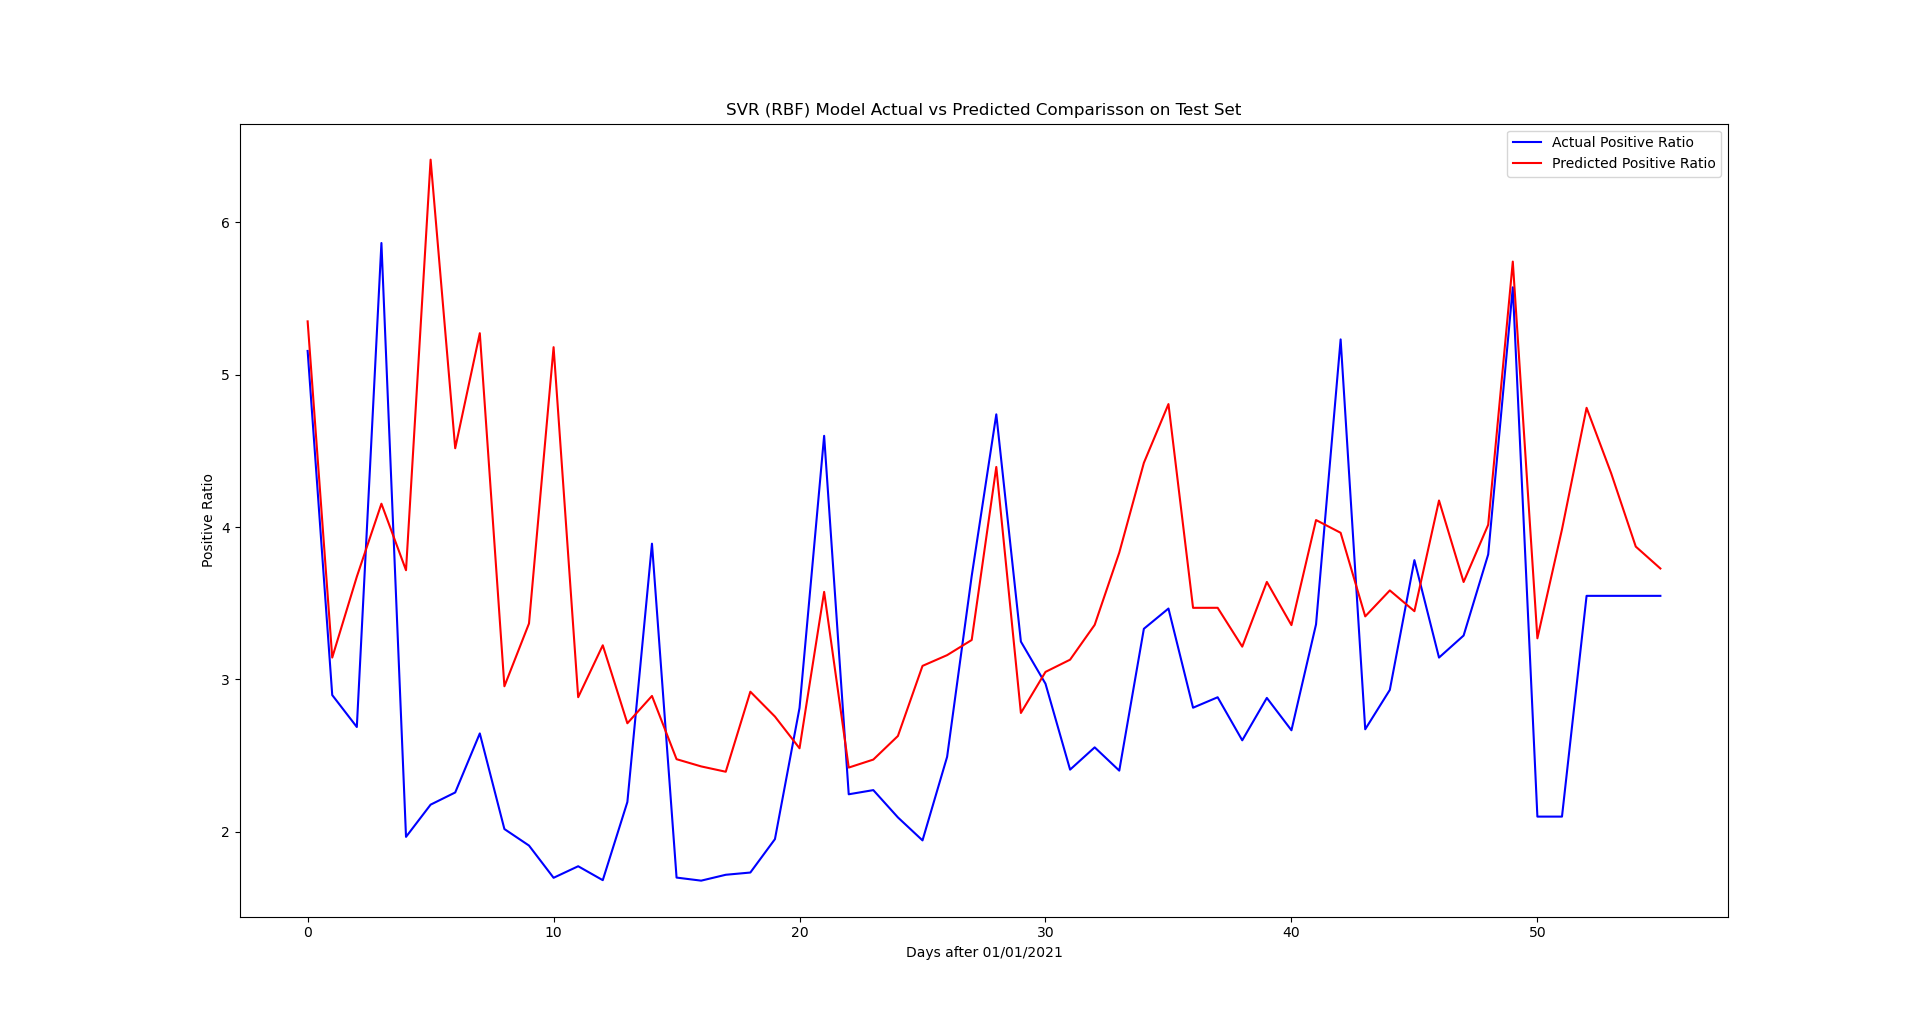
\includegraphics[width=\textwidth]{Figures/Question3/1. SVR Actual vs Predicted Test Set.png}
	\caption{SVM - Σύγκριση κανονικών τιμών και τιμών πρόβλεψης για το validation με το test set}
\end{figure}

\begin{figure}[H]
	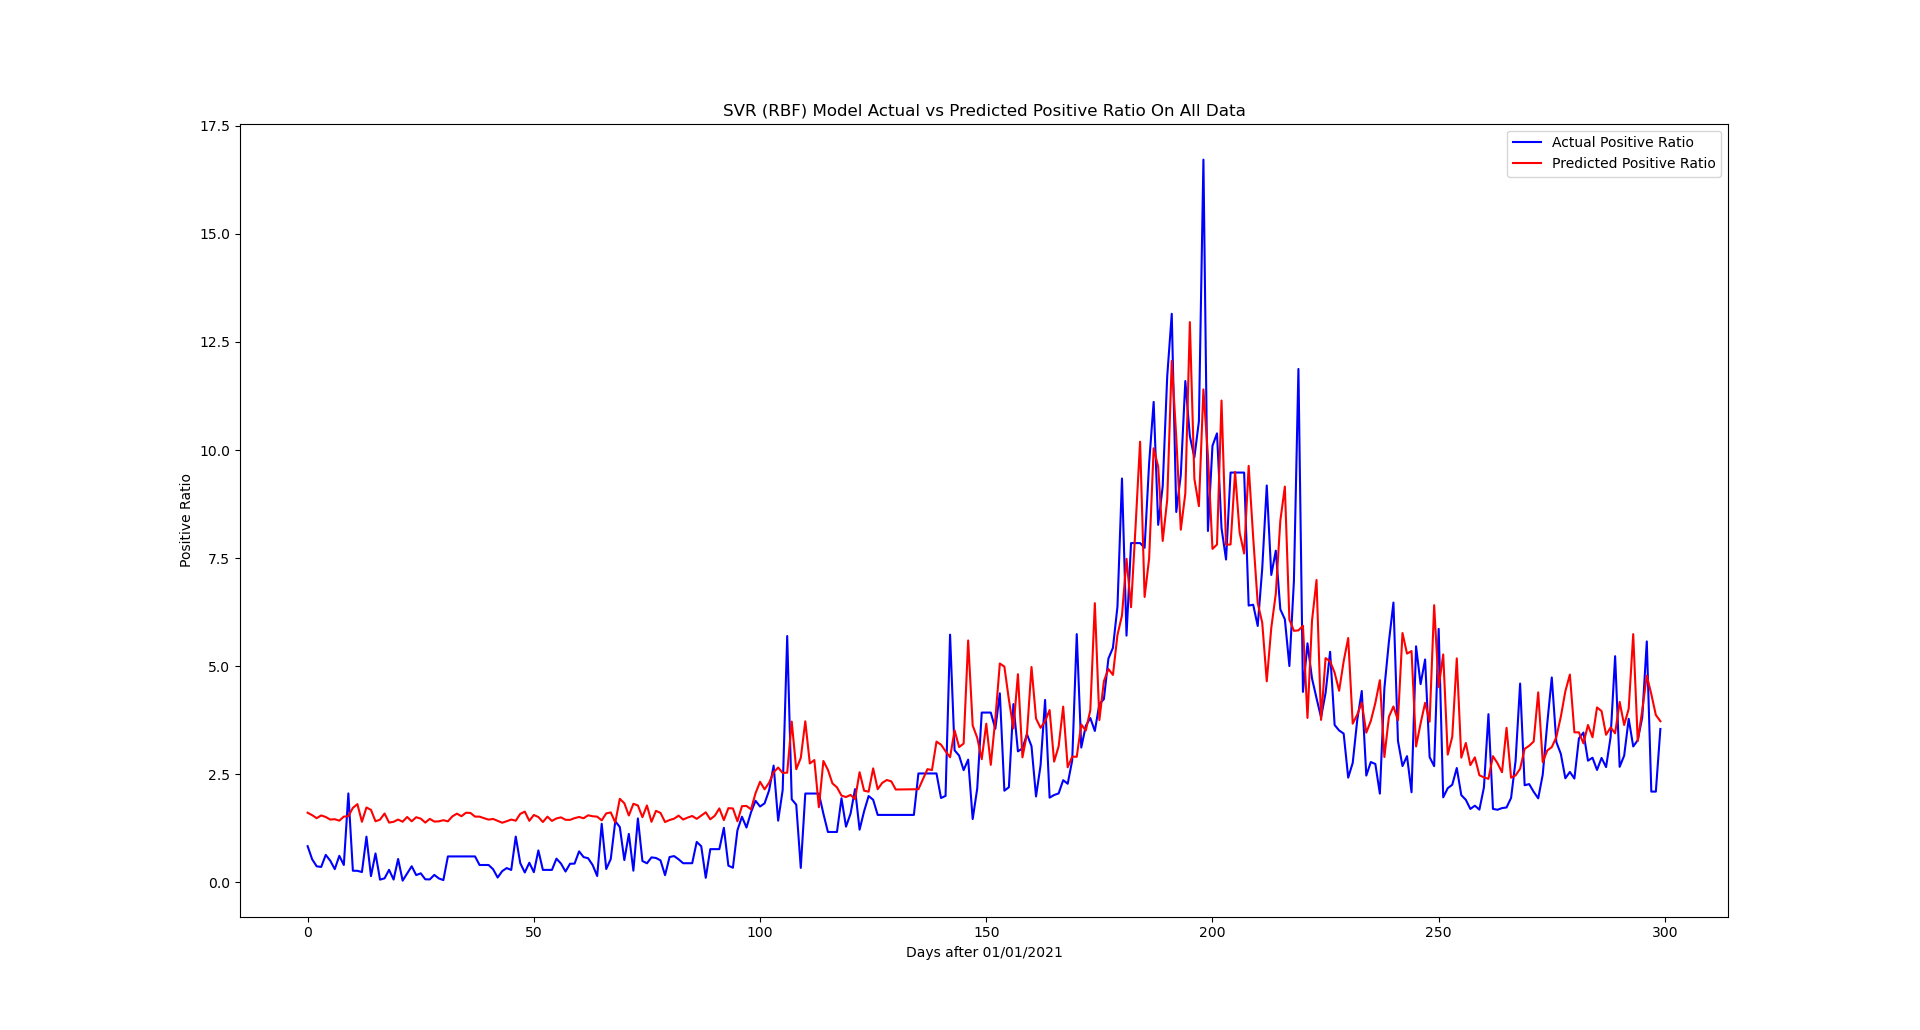
\includegraphics[width=\textwidth]{Figures/Question3/2. SVR Actual vs Predicted All Data.png}
	\caption{SVM - Σύγκριση κανονικών τιμών και τιμών πρόβλεψης για όλα τα δεδομένα (για ένδειξη)}
\end{figure}

\subsubsection{Αποτελέσματα RNN βασισμένου μοντέλου}

Παρακάτω παρουσιάζουμε τις μετρικές σφάλματος και αξιολόγησης (MSE και MAPE) ανά εποχή στο train set και test set, καθώς και τις τελικές τιμές MSE και MAPE στο evaluation με το test set. Επίσης παρουσιάζουμε και τις γραφικές των prediction, όπως κάνουμε και παραπάνω.

\textbf{Evaluation MSE\textsubscript{Actual vs Predicted} =} 0.0039

\textbf{Evaluation MAPE\textsubscript{Actual vs Predicted} =} 25.4686

\begin{figure}[H]
	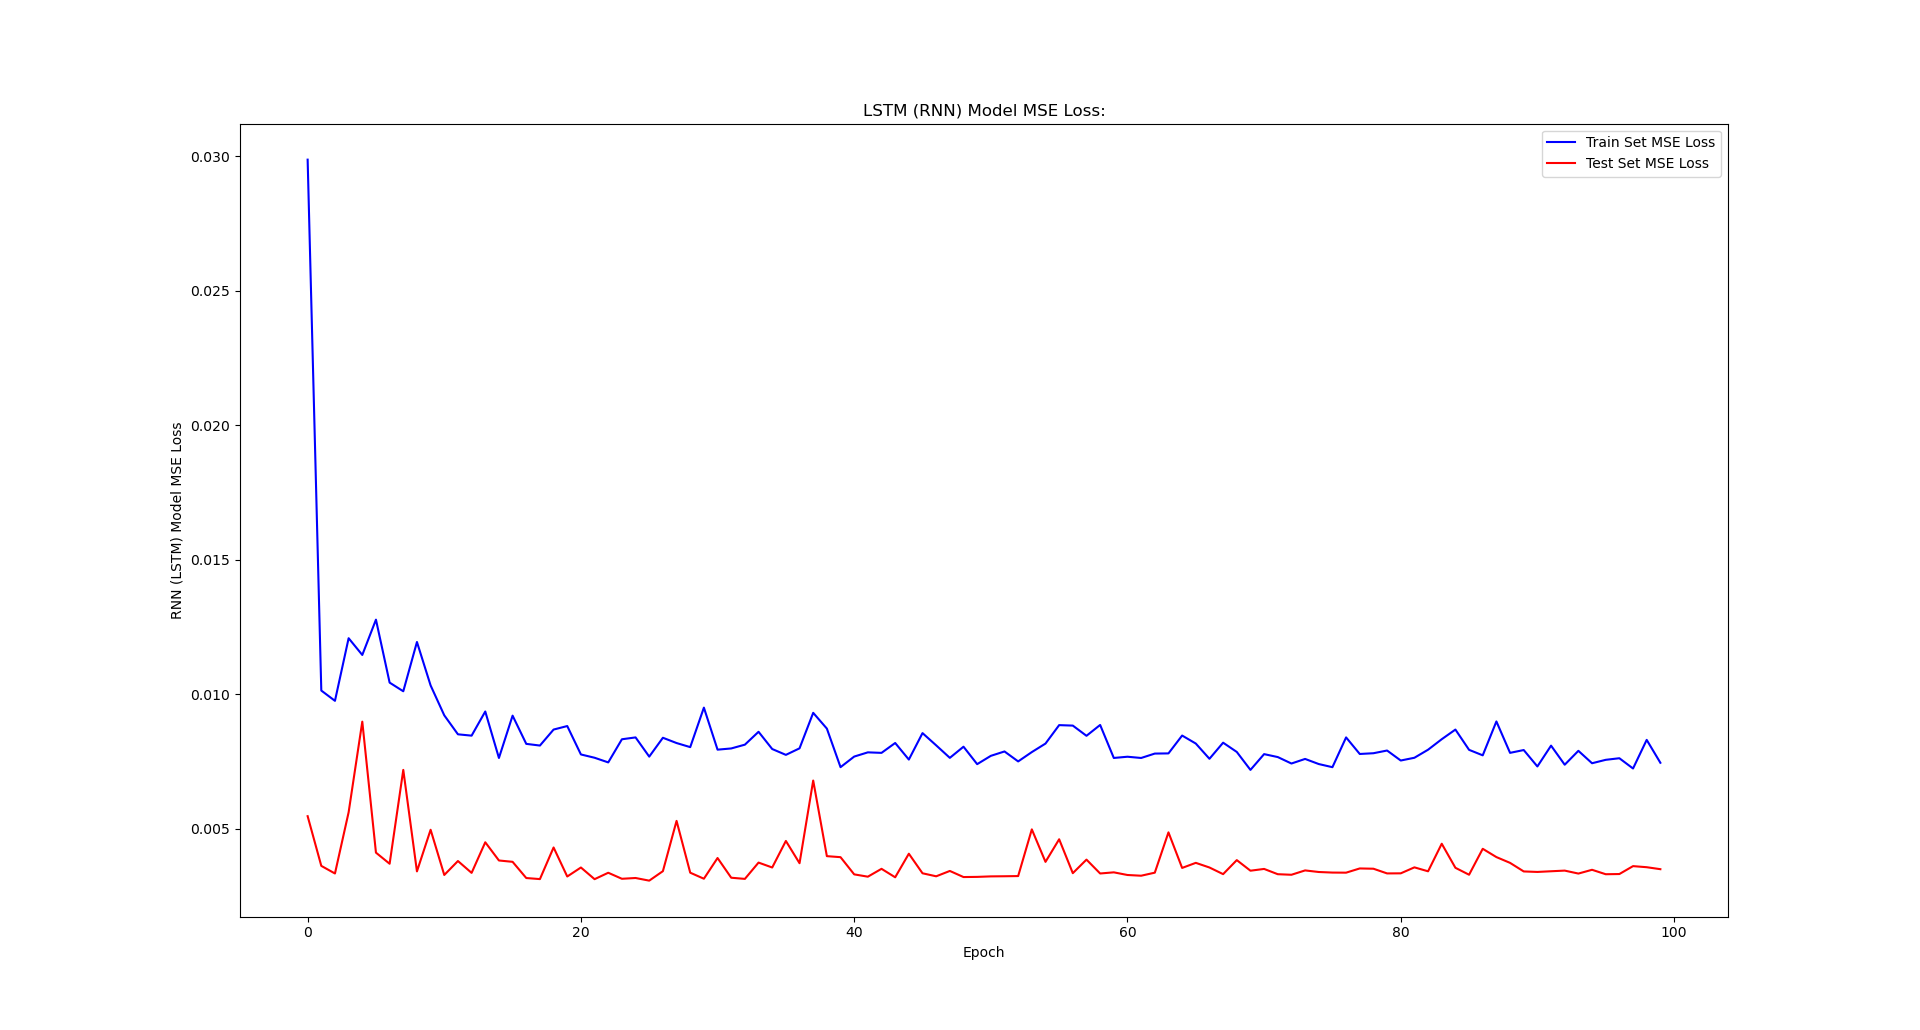
\includegraphics[width=\textwidth]{Figures/Question3/3. RNN Model MSE Loss.png}
	\caption{RNN - MSE ανά εποχή για train και test set}
\end{figure}

\begin{figure}[H]
	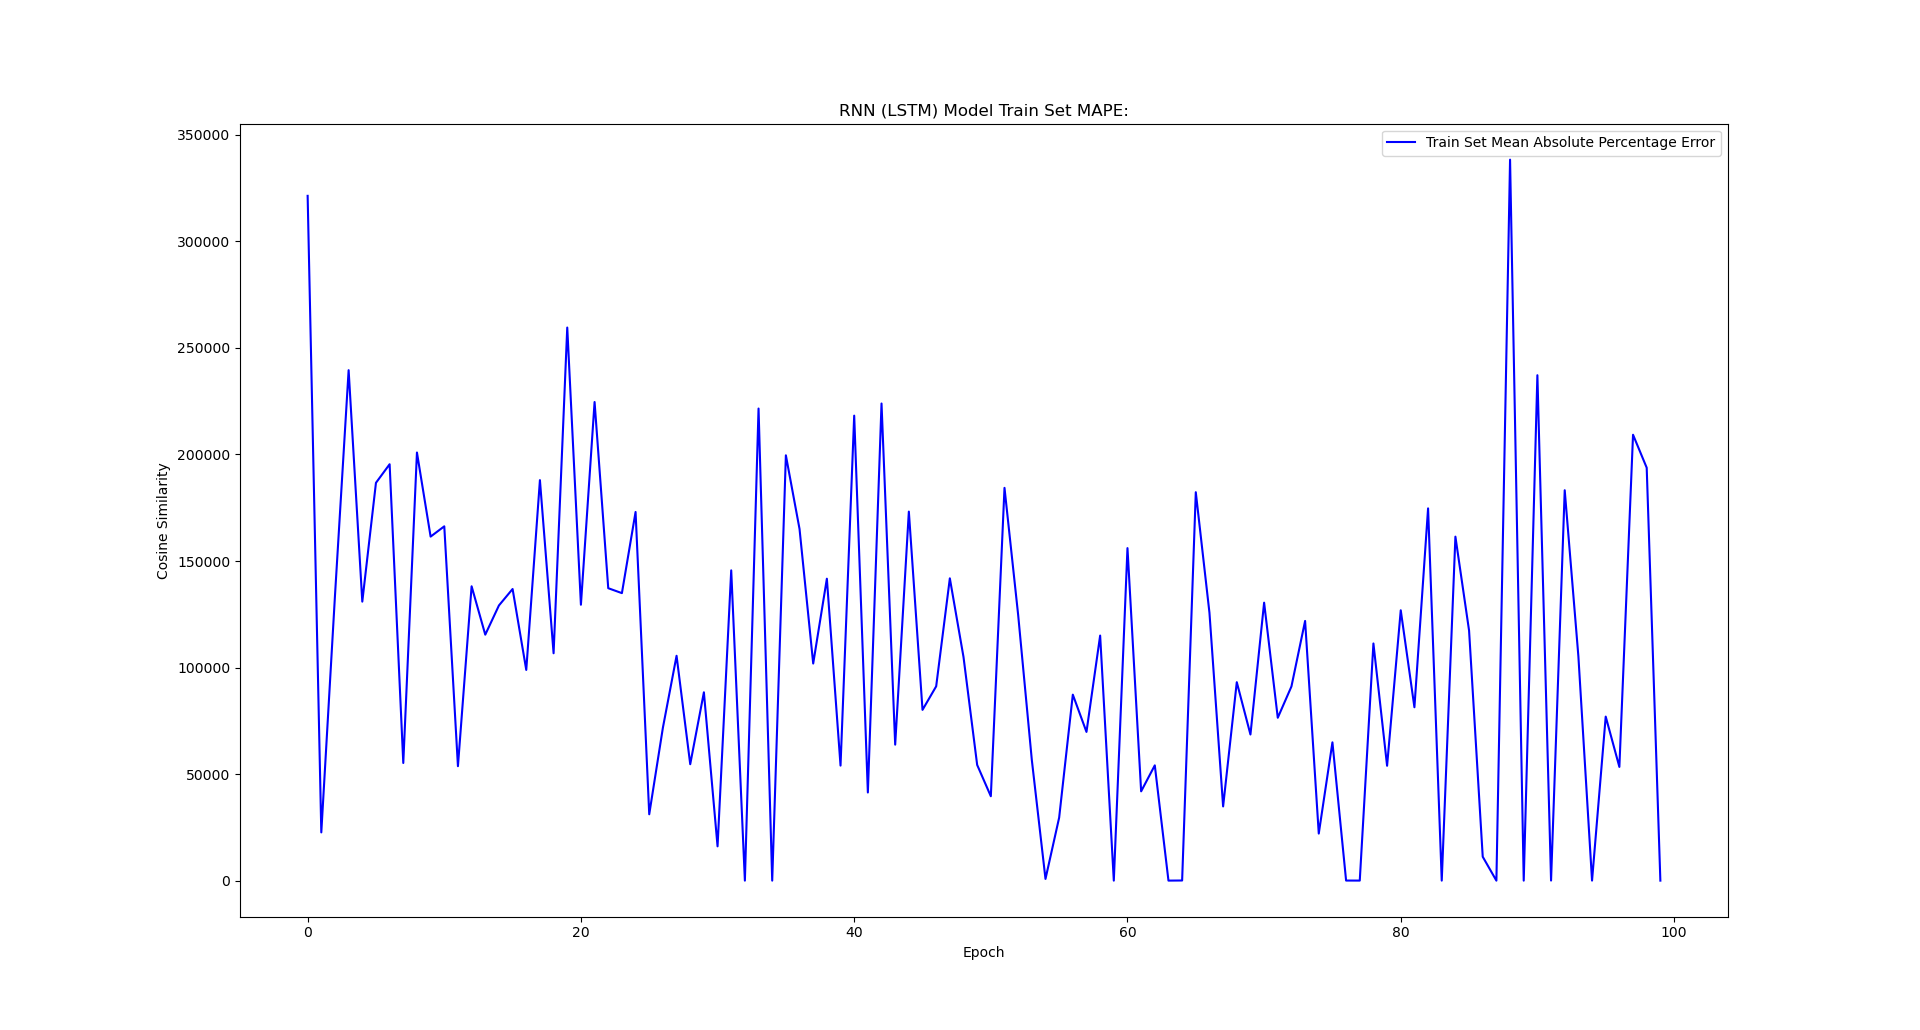
\includegraphics[width=\textwidth]{Figures/Question3/4. RNN Model Train MAPE.png}
	\caption{RNN - MAPE ανά εποχή για train set}
\end{figure}

\begin{figure}[H]
	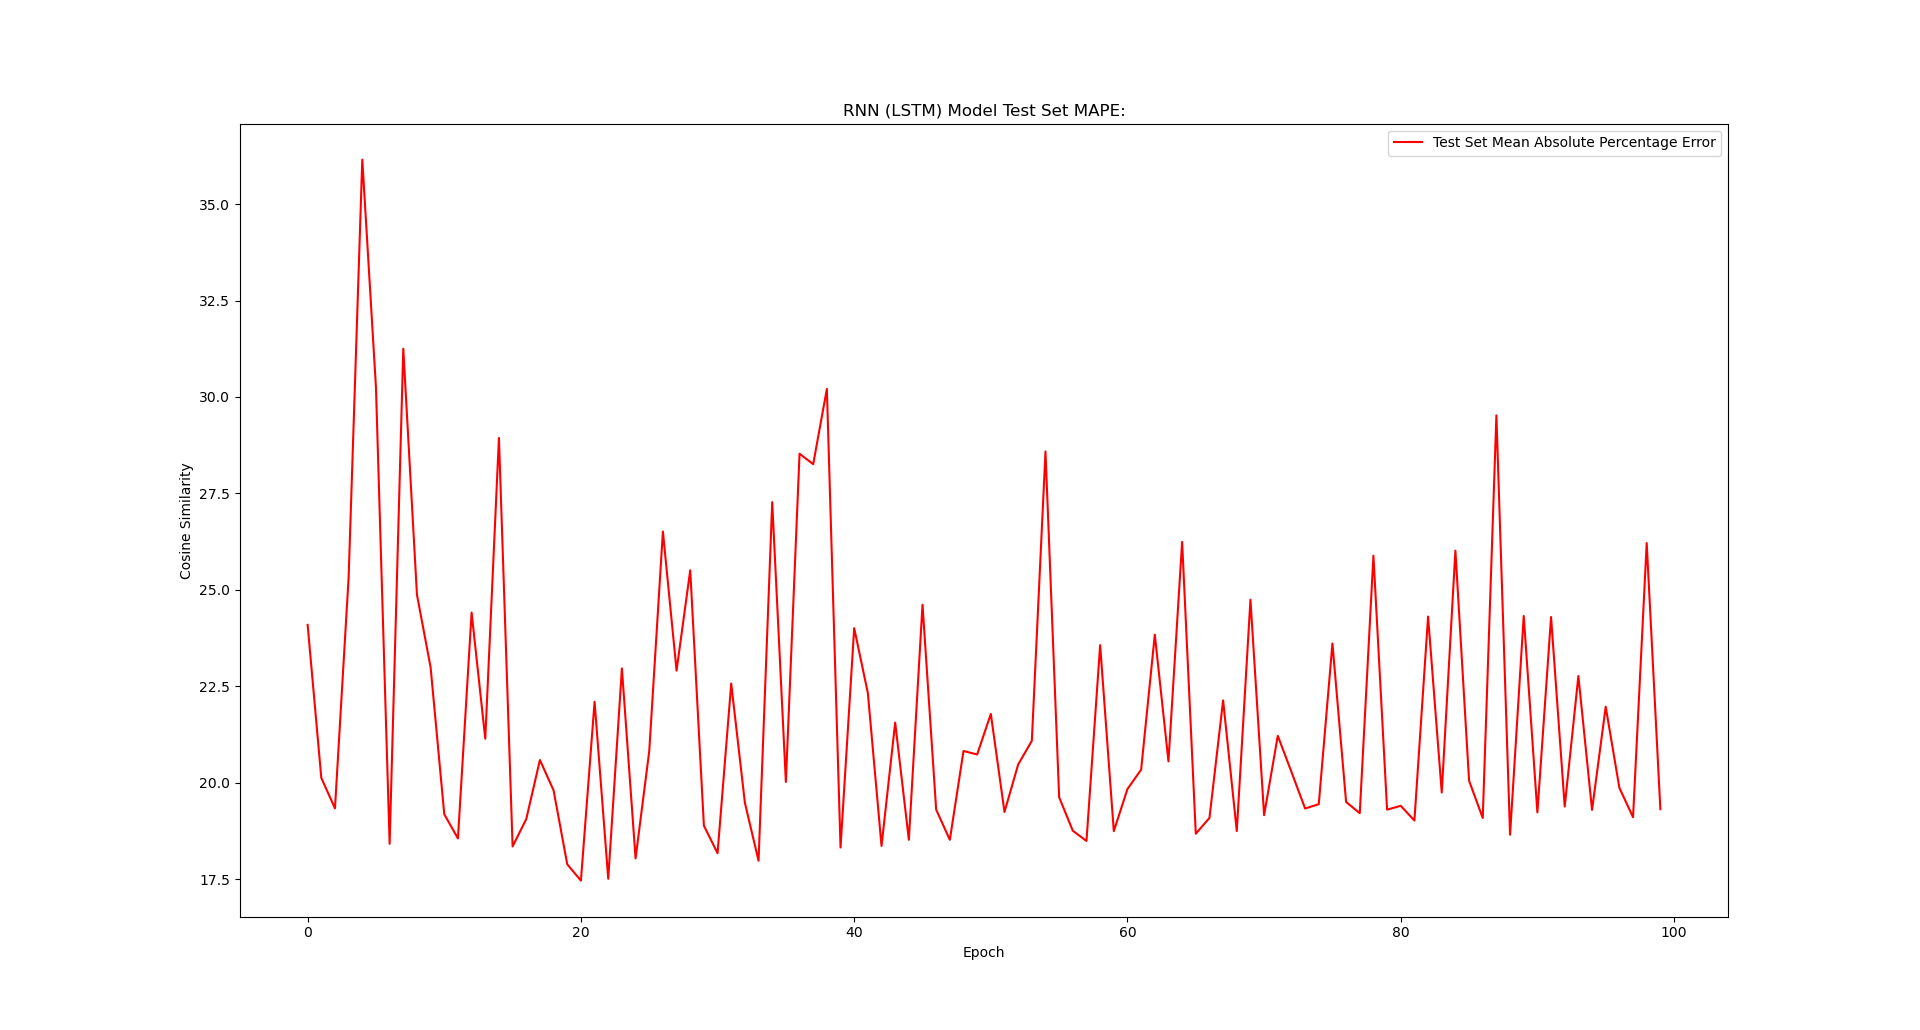
\includegraphics[width=\textwidth]{Figures/Question3/5. RNN Model Test MAPE.png}
	\caption{RNN - MAPE ανά εποχή για test set}
\end{figure}

\begin{figure}[H]
	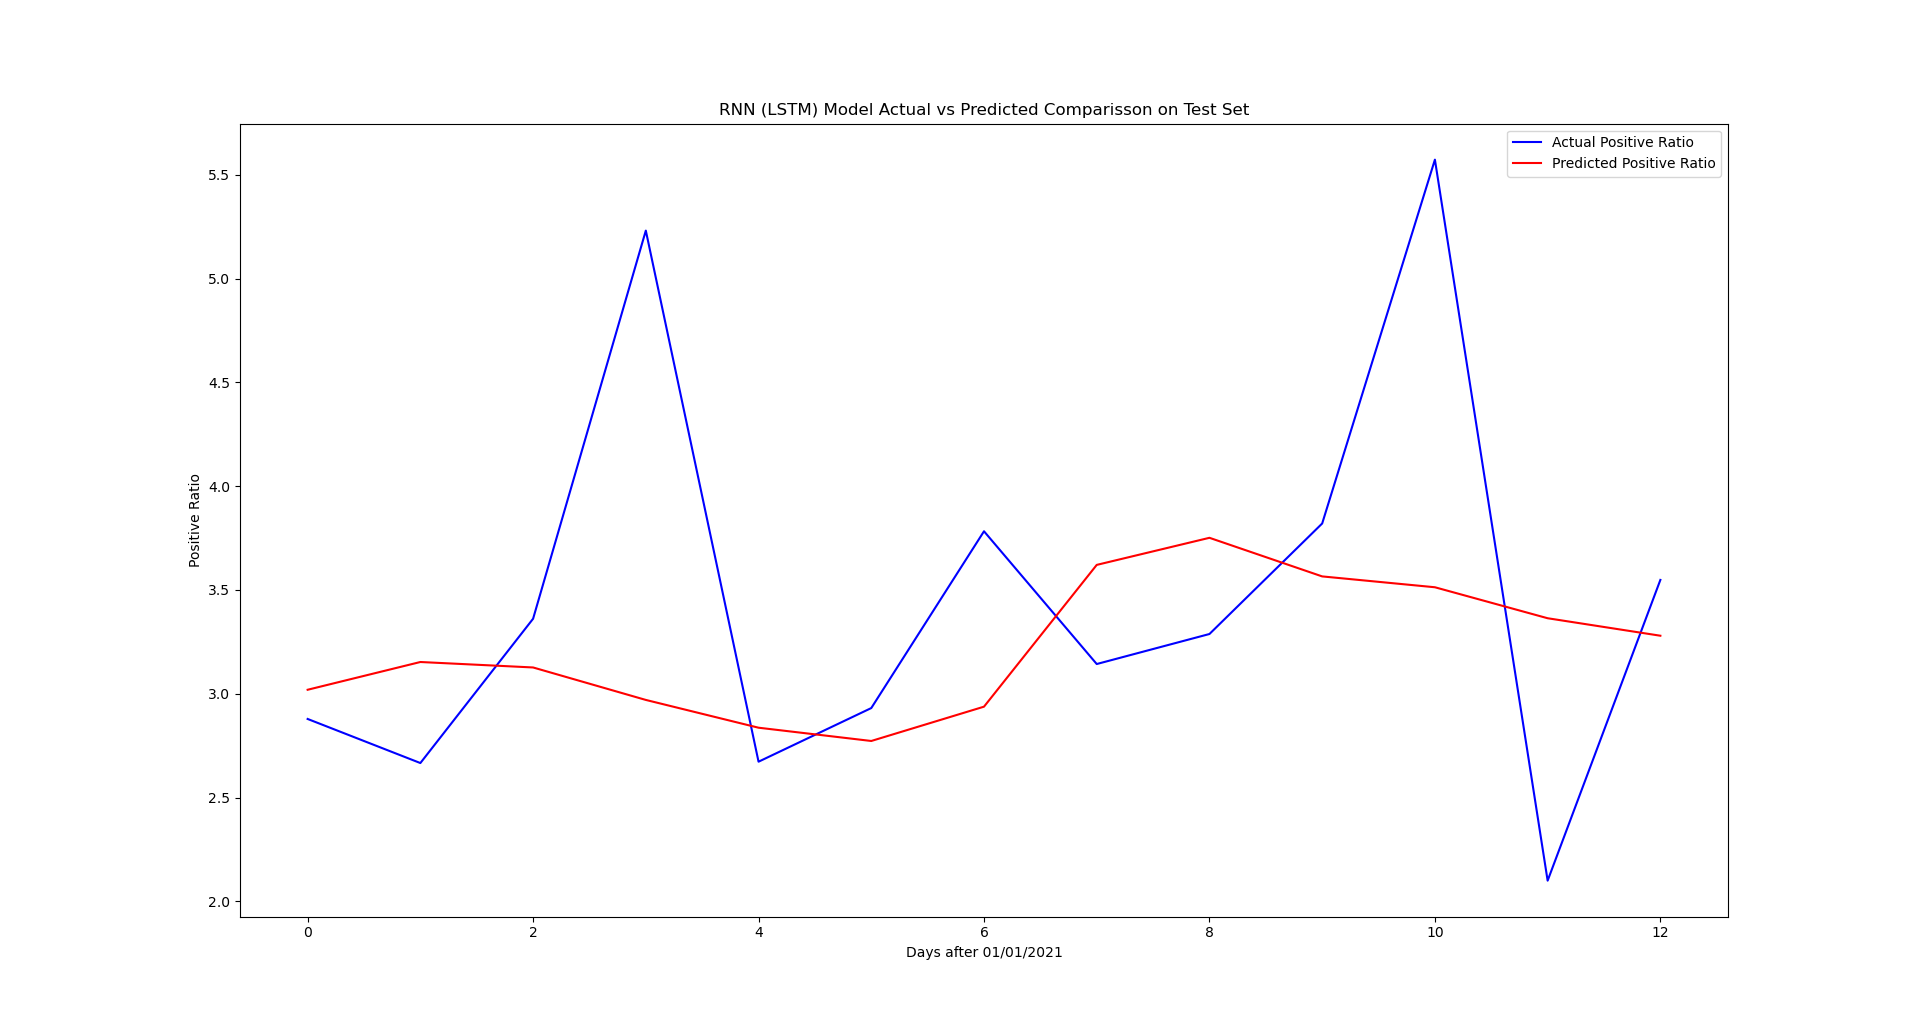
\includegraphics[width=\textwidth]{Figures/Question3/6. RNN Actual vs Predicted Test Set.png}
	\caption{RNN - Σύγκριση κανονικών τιμών και τιμών πρόβλεψης για το validation με το test set}
\end{figure}

\begin{figure}[H]
	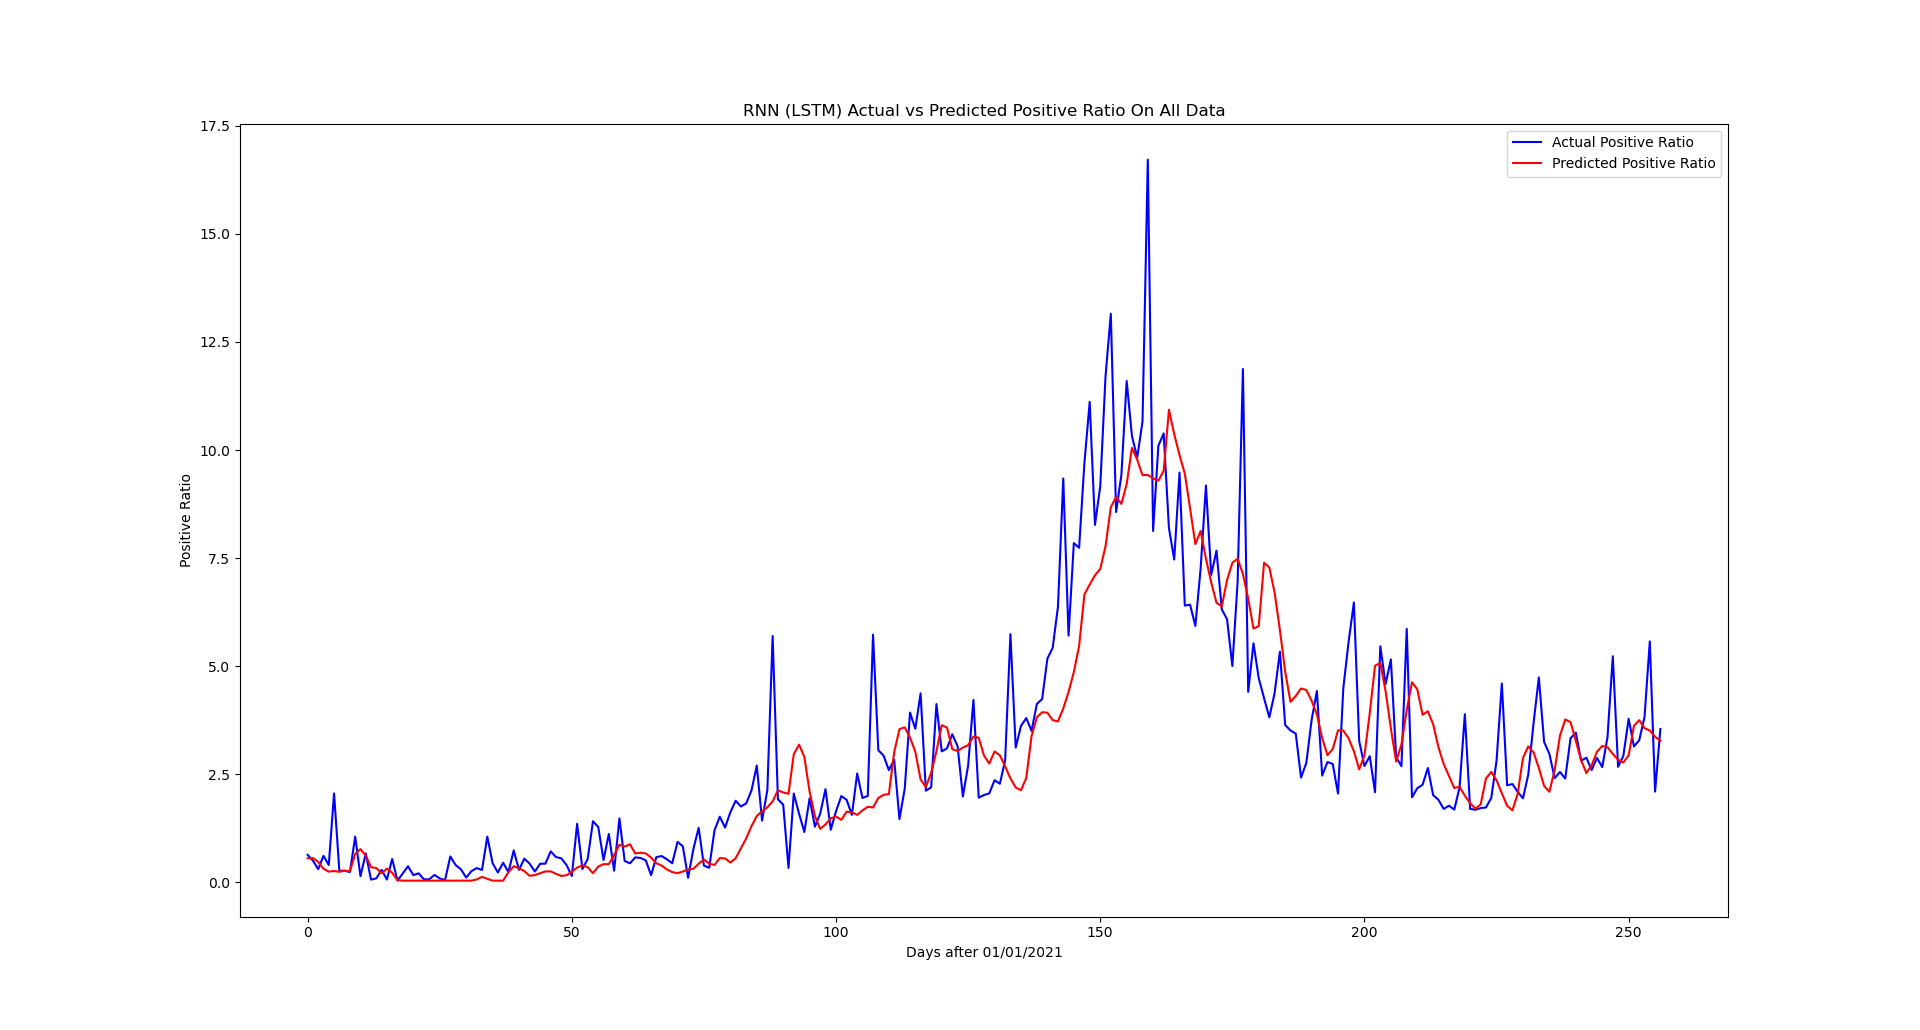
\includegraphics[width=\textwidth]{Figures/Question3/7. SVR Actual vs Predicted All Data.png}
	\caption{RNN - Σύγκριση κανονικών τιμών και τιμών πρόβλεψης για όλα τα δεδομένα (για ένδειξη)}
\end{figure}

\subsubsection{Συμπεράσματα}

Αρχικά παρατηρούμε από τις τιμές του MSE των validations με τα test set ότι η λύση με το RNN έχει καλύτερη ακρίβεια στις προσεγγίσεις της πραγματικής τιμής του 'Positivity Rate'. Το ίδιο παρατηρείται και οπτικά στα prediction που γίνονται σε όλα τα δεδομένα. Ταυτόχρονα παρατηρούμε ότι οι προβλεπόμενες τιμές των RNN έχουν μικρότερους ρυθμούς εναλλαγών τιμών από ότι την υλοποίηση με τα SVM.

Επίσης στα predictions όλων των δεδομένων παρατηρούμε ότι δεν υπάρχει καθαρή διαφορά ή εναλλαγή μεταξύ train και test set, που σημαίνει ότι τα μοντέλα γενικεύουν και αποδίδουν και για νέα δεδομένα (αν το μικρό test set είναι αντιπροσωπευτικό για το σύνολο των δεδομένων του πραγματικού κόσμου).

Τέλος στη γραφική παράσταση του MSE ανά εποχή στο test και train set για το παράδειγμα των RNN παρατηρούμε αρχικά ότι ο ρυθμός βελτίωσης της απόδοσης μετά από σχετικά μικρό αριθμό εποχών (20 περίπου) είναι σταθερός. Επειδή όμως δεν υπάρχει σημαντική μείωση του σφάλματος στο train set και ούτε αύξηση σφάλματος στο test set δεν θεωρούμε ότι γίνεται overfitting, στο οποίο συμβάλλει και η χρήση των dropout layers. 

Παρόλα αυτά βέβαια δεν υπάρχει ούτε αύξηση της επίδοσης, οπότε θα μπορούσε σε αυτή τη περίπτωση να είχε σταματήσει το training σε μικρότερο αριθμό εποχών, αλλά επειδή ο ιδανικός αριθμός εποχών παρουσιάζει τυχαιότητα και πολλές φορές το early stopping μπορεί να σταματήσει νωρίς το training, καθώς και δεν γίνεται overfitting προτιμήσαμε ένα αυθαίρετα μεγάλο αριθμό εποχών στη περίπτωση αυτή.

Επίσης παρατηρείται ότι το test set έχει πάντα μικρότερο σφάλμα από το train set, το οποίο συμβαίνει επειδή οι τιμές στο test set έχουν μικρότερο εύρος τιμών από ότι αυτές στο train set και παρουσιάζουν μικρότερες διακυμάνσεις, οπότε είναι "πιο εύκολο" για το μοντέλο να τις προβλέψει.

\textbf{Σημείωση:} Εκτός από τη προσέγγιση χρήσης των δεδομένων του 'Positive Ratio' των 6 τελευταίων ημερών για την πρόβλεψη, όπως εξηγήσαμε και παραπάνω, έχουμε δοκιμάσει και εναλλακτικές μεθόδους, όπως την χρήστη όλων των δεδομένων (όλα τα Series) των 6 τελευταίων ημερών και τη χρήση όλων των δεδομένων για τη τελευταία ημέρα. Παρατηρήσαμε όμως πως η προσέγγιση που εξηγήσαμε παραπάνω παρουσίαζε τα καλύτερα αποτελέσματα οπότε δεν εξηγήσαμε τις άλλες, παρόλα αυτά παρέχονται και αυτά σε μορφή κώδικα στο GitHub στο φάκελο 'Code/Extras - Different Tested Approaches'.

\end{document}
